\chapter{Materialien}
\label{ch:materialien}

\section[Das \tit{Corpus der altdeutschen Originalurkunden}]{Das \tit{Corpus der
altdeutschen Originalurkunden}}%{Das \citetitle*{cao}}
\label{sec:materialcao}

Das \citetitle*{hrg} definiert den Terminus \q*{Urkunde} als
\blockcquote[574]{frenz1998a}{schriftliche Aufzeichnung über einen Vorgang
rechtlicher Natur, die unter Beachtung gewisser Formen geschieht und in einer
bestimmten Weise beglaubigt ist; die U\textins{rkunde} will eine rechtliche
Wirkung erzielen und erhebt den Anspruch der Glaubwürdigkeit}. Diese Kriterien
unterscheiden sie von anderen formal ähnlichen Quellengattungen, wie zum
Beispiel Akten oder Briefen. Nicht zu verwechseln mit letzerem ist mhd.\
\norm{brief}, mit dem nicht nur Briefe, sondern auch Urkunden bezeichnet
werden, neben \norm{hantvėste} \autocites[][\pno~\fw{brief},
]{mwb1}[][\pno~\fw{hantveste}]{mwb2}[vgl. auch][]{schmidtwiegand1998a}.
% \cref{ex:bspurkunde} zeigt als Beispiel eine Urkunde, die 1289 in Wien
% ausgestellt wurde \autocite[\pno~1073]{cao2}.
% 
% \begin{figure}
% \centering
% \includegraphics[
% 	height=.60\textheight
% ]{./assets/grafiken/CAO_01073-bearbeitet.jpg}
% \caption%
% 	[Heiligenkreuz, Stiftsarchiv, Wien St. Nikolaus, Urkunden 1289]%
% 	{Heiligenkreuz, Stiftsarchiv, Wien St. Nikolaus, Urkunden 1289
% 		(Foto: Monasterium.net)}
% \label{ex:bspurkunde}
% \end{figure}

Das \citetitle{cao} umfasst 4.617 Originalurkunden aus dem 13.\ Jahrhundert
(das heißt keine zeitgenössischen oder späteren Abschriften), davon sind 4.289
deutschsprachig. Daneben existieren in weitaus geringerem Maße Urkunden auf
Mittelniederländisch und Latein
\autocites[\RN{1}]{deboor1976}[25]{schulze2011}[40--41]{ganslmayer2012}.%
%
	\footnote{\citet[391]{gniffkerapp2005} geben die Gesamtzahl an Urkunden,
	die das \citetitle{cao} versammelt, mit 4.422 an. Die Diskrepanz in der
	Zählung ergibt sich dadurch, dass Parallelausfertigungen von ihnen nicht
	mitgezählt wurden
	\autocite[vgl.][40]{ganslmayer2012}.\label{fn:caowordcount}}
%
Beim Inhalt des \citetitle{cao} handelt es sich nicht nur um Urkunden im
engeren Sinn \autocite[596]{schmidtwiegand1998b}. So sind gerade für die
Frühzeit in der ersten Hälfte des 13.~Jahrhunderts neben dem \tit{Erfurter
Judeneid} \autocite[1]{cao1} und der \tit{Venusfahrt} aus dem
\tit{Frauendienst} Ulrichs von Liechtenstein \autocite[3]{cao1}%
%
	\footnote{Vgl.\ München, Bayerische Staatsbibl., Cgm~44, Bl.~36\va--37\rb{}
	\autocite[1307]{hsc}.}
%
auch diverse Stadtrechte enthalten, beispielsweise die von Braunschweig und von
Straßburg \autocites[2]{cao1}[N~238~AB]{cao5}, sowie als ältester
überlieferter deutschsprachiger Rechtstext der \tit{Mainzer Reichslandfrieden}
von 1235 in mehreren Fassungen \autocite[4]{cao1}.%
%
	\footnote{Neben zwei lateinischen Fassungen \autocite[\ppno~4~Dor,
	4~F]{cao1} handelt es sich dabei um die folgenden Handschriften, die den
	Text auf deutsch in späteren Abschriften überliefern -- hier wurde eine
	Ausnahme vom Prinzip der \q*{Originalurkunde} gemacht:

	\begin{tabularx}{\linewidth}{@{} l >{\citereset}X @{}}
	D & Dresden, Sächsische Landesbibl., Mscr.Dresd.M.32: Bl.~1\ro\vo; Mitte 14.\ Jh.
		\autocite[7549]{hsc}
	\\

	P & München, Bayerische Staatsbibl., Clm~16083: Bl.~2\ro; Mitte
		13.\ Jh. \autocites[256]{haas2010}[19293]{hsc}
	\\
	W & Wolfenbüttel, Herzog August Bibl., Cod.~3.1~Aug.~2°: Bl.~1\ro--3\vb;
		3.~Viertel 14.~Jh. \autocite[8396]{hsc}
	\\
	\end{tabularx}

	Um frühe Originalurkunden im engeren Sinn handelt es sich bei den
	Nrn.~6--9 und 39 \autocites{cao1}[vgl.][15--16]{bertelsmeierkierst2008}.%
	}
%
Bei den meisten im \citetitle{cao} enthaltenen Texten handelt es sich um
Privaturkunden, insofern diese nicht von Kaisern oder Königen
% oder Päpsten
ausgestellt wurden
% -- letztere urkundeten ohnehin nicht auf Deutsch
\autocites[vgl.][575]{frenz1998a}[585]{frenz1998b}. Einen Eindruck von der
enormen Variationsbreite der verhandelten -- vor allem sehr alltagsnahen --
Gegen\-stände geben \textcites[11]{schulze2011}[35--36]{ganslmayer2012}.
%
% \blockcquote[11]{schulze2011}{Es geht um geistliche und weltliche Herren
% unterschiedlichen Ranges, um Städte und Klöster, Bürger, Kaufleute,
% Handwerker, Juden, freie und abhängige Bauern, Mönche, Nonnen, Kreuzfahrer,
% Männer und Frauen, Verstorbene und Lebende, Menschen und Tiere; es geht um
% Kirchen, Burgen, Dörfer, Ländereien mit Äckern, Wäldern, Wiesen, Baumgärten,
% Weinbergen, Bergwerken, Mühlen, um den Verkehr zu Wasser und zu Lande, um
% Salz, Eicheln, Bucheln, Hühner, Käse, Schinken, Krapfen, Kerzen, Rüstungen,
% Schuhe mit hohen Absätzen, Geld in verschiedenster Währung,
% Abwasserverschmutzung, Bierbrauen, Brotbacken, Brandstiftung,
% Klostereintritt, Glockenläuten, Messe-Singen, um eine Vielzahl von
% Tätigkeiten, um konkrete und abstrakte Beziehungen.}
%
Auch die Thematik der verschiedenen Urkunden ist
breit: \blockcquote[596]{schmidtwiegand1998b}{\textins{So} handelt es sich im
übrigen um Anweisungen, Verträge, Abmachungen, Geschäfte, Streitigkeiten und
deren Regulierungen seitens weltlicher und geistlicher Herren unterschiedlichen
Ranges, Institutionen wie Städten und Klöstern, Bürgern, Kaufleuten und
Handwerkern, freien und abhängigen Bauern, Mönchen, Nonnen und Kreuzfahrern.}

Das \citetitle{cao} ist ein Produkt jahrzehntelanger Sammeltätigkeit. Friedrich
Wilhelm\nocite{wilhelm1932} (1882--1939)%
% Quelle: https://d-nb.info/gnd/117380814
% Quelle: \autocite[2031]{bubenik2003}
, sein Begründer, verfolgte von Anfang an das Ziel, ein Textkorpus
bereitzustellen, das nicht durch Normalisierung, also sprachliche Glättung und
Vereinheitlichung \autocites[vgl.][76--84]{bein2011}{kragl2015},
\blockcquote[\RN{60}]{wilhelm1932}{für den Sprachforscher unbrauchbar} gemacht
wurde. \posscite[161]{lachmann1820} ästhetischem Ideal von
\blockcquote[\RN{3}]{wilhelm1932}{jenem \q{unwandelbaren Hochdeutsch}, das
\q{die Dichter des dreizehnten Jahrhunderts bis auf wenig % \textins{sic}
mundartliche Einzelheiten \textelp{} redeten} \textelp{}, welches in seiner
sauberen Gleichmäßigkeit dem Latein klassisch-philologischer Schulausgaben
glich, und das \textelp{} nicht Eingeweihten ein Idealbild vorgaukelte} setzt
er konsequent und mit polemischer Schärfe sein Credo des möglichst
originalgetreuen Abdrucks entgegen.

% \citeauthor{wilhelm1932} schildert mit bitteren Worten, wie seine Zeitgenossen
% dem Projekt kritisch bis ablehnend gegenüberstanden
% \autocite[\RN{75}--\RN{80}]{wilhelm1932}. Jedoch änderte sich mit der Zeit die
% Einstellung der Forschergemeinschaft gegenüber dem Wert einzelner
% Textträger, sodass nach dem Zweiten Weltkrieg bereitwillig Gelder gewährt
% wurden, das Projekt unter der Ägide von Richard Newald sowie seiner
% Nachfolgerinnen und Nachfolger weiterzuführen
% \autocite[\RN{11}--\RN{12}]{deboor1976}.
In seinem \citetitle{deboor1976} zum abschließenden fünften Band des
\citetitle{cao} hebt \citeauthor{deboor1976} versöhnlich hervor, dass heute
niemand \blockcquote[\RN{13}]{deboor1976}{mehr bestreiten \textins{wird}, daß
die großen kritischen Ausgaben Karl Lachmanns und seiner Nachfolger für die
Forschung nötig und segensreich waren}, indem sie alte Texte überhaupt wieder
zugänglich und vermittelbar gemacht und damit wissenschaftliches Interesse
geweckt haben. Gegen die Frage der Editionsphilologie nach der Genese,
Überlieferung und Rekonstruktion von Texten ist nichts einzuwenden.

Darüber hinaus sind normalisierte Formen auch in linguistischer Hinsicht
nützlich, da sie sich unabhängig von individuellen Grafien in
unterschiedlichen Textzeugen als Zitations\-formen eignen. Moderne technische
Möglich\-keiten können die Anforderungen beider Parteien, der
Literaturwissenschaft und der historischen Linguistik, erfüllen, was das
Spannungsfeld zwischen Lesbarkeit, Textkritik und Datentreue betrifft, zumal
auch die moderne Editionstätigkeit radikales \q*{Glattbügeln} von Texten, wie
\citeauthor{wilhelm1932} es seinen Zeitgenossen vorwarf, durch das heute
größere Interesse an der Materialität der Textüberlieferung eher scheut
% \autocite[vgl.][144]{chincaetal2019a}.
\autocite[vgl.][1306]{wegera2000}.%
%
	\footnote{Zum Beispiel stellt das Projekt \citetitle{ldmdigital} von
	\citet{ldmdigital} neben der diplomatischen Transkription mit dynamisch
	einblendbaren Abkürzungsauflösungen den normalisierten Editionstext der
	einzelnen Lieder zur Verfügung, sodass ein direkter Vergleich zwischen
	Handschrift, Transkription und Edition möglich ist, siehe
	\urlcite{ldmdigital}. Die in den vergangenen Jahren aufgebauten
	historischen Referenzkorpora des Deutschen
	(z.\,B. \cite{ddd}, \cite{rem}; \cite[vgl.][522--523]{dipper2015}) bieten neben
	diplomatischen Transkriptionen ebenfalls normalisierte Versionen der
	jeweiligen Textzeugen als Annotations- bzw.\ Abstraktionsschicht.}

Dem Geist \citeauthor{wilhelm1932}s folgend betonen sowohl \citet{deboor1976}
als auch \citet{schulze2011} besonders den Wert des \citetitle{cao} als
Korrektiv gegenüber den mittelhochdeutschen Grammatik\-darstel\-lungen wie zum
Beispiel der von \citet{paul2007}. So schreibt \citet[22]{schulze2011}, dass
zwar \textquote{\textins*{d}ie Vorbehalte gegenüber der Urkundenauswertung
\textelp{} inzwischen weitgehend geschwunden} seien. Zum damaligen Zeitpunkt
waren aber nach wie vor \blockcquote[22]{schulze2011}{\textins*{w}ichtige
Aspekte zur mittelhochdeutschen Grammatik \textelp{} nicht primär auf
sprachgeografische Zuordnungen ausgerichtet. Bei syntaktischen Untersuchungen
verschiedener Art gibt es viele übergreifende Fragen und Beobachtungen, für die
das besondere Quellenmaterial ergiebig ist und die allenfalls zusätzlich
sprachgeographisch weiter differenziert werden können.} Auch
\citet{wegera2000} bemerkt kritisch, dass in den Grammatiken des
Mittelhochdeutschen nach Paul\nocite{paul2007} und \citeauthor{mettke1993}
\blockcquote[1305]{wegera2000}{\textins*{k}eine der Textsammlungen adäquat die
regionale Variabilität oder die Diachronie von drei Jahrhunderten
wider\textins*{spiegelt}, noch \textelp{} eine Textsortenspezifik sichtbar
\textins*{wird}. Den Schwerpunkt bilden in allen Fällen die poetischen
Denkmäler des späten 12.\ und frühen 13.~Jhs.\ obd.\ Provenienz. Einige
wenige Urkunden und andere Prosatexte \textelp{} werden zwar genannt, doch bei
der Auswertung kaum berücksichtigt.}

Das Textkorpus zur neuen \tit{Mittelhochdeutschen Grammatik}
von \citet{ksw3,ksw2} versucht hier gegenzusteuern durch ein bezüglich Zeit,
Sprachräumen und Textsorten sorgfältig ausbalanciertes Textkorpus, das auf
repräsentativen Exzerpten möglichst von Original\-handschriften basiert
\autocites[1311--1318]{wegera2000}[3]{kleindipper2016}. Auch Urkunden sind Teil
dieses Korpus, doch nur zu einem relativ geringen Teil. In den 103 gelisteten
Quellen des Grammatik-Korpus \autocite%
	% s[19--30]{ksw3}%
	[14--26]{ksw2}
sind die zehn in \cref{tab:kswurk} aufgeführten Urkundenstrecken mit insgesamt
225 Urkunden enthalten. Dabei werden für das 13.~Jahrhundert das Hessische,
Rheinfränkische, Ostmitteldeutsche, Bairische und Ostfränkische aufgrund der
Aufnahmebedingungen nicht abgedeckt \autocite[vgl.][1311]{wegera2000}. Da auch
für die abgedeckten Dialektregionen Mittelfränkisch, Alemannisch und Schwäbisch
jeweils nur eine große Stadt als Schreibzentrum aufgenommen wurde, ist kritisch
zu fragen, ob die Auswahl für das 13.~Jahrhundert tatsächlich repräsentativ
ist.%
%
	\footnote{Die einzelnen enthaltenen Texte können
	\citet[Textübersicht]{kleindipper2016} entnommen werden. Laut dieser Liste
	sind aus dem \citetitle{cao} enthalten: Nrn.~53, 60, 61, 71, 72~AB, 74,
	75, 76, 78, 79, 83, 85, 223, 224, 428, 429, 508, 548~AC, 549, 560, 658,
	677, 780, 831, 1371, 1542, 1639, 1648, 1651~B, 1678, 1686, 1768, 1883,
	1958, 1959, 1985, 2001, 2008, 2112, 2133, 2182, 2277, 2348, 2461, 2643,
	2681, 2725, 2733, 2767, 2780, 2861, 2909, 2921, 2936, 3018, N~36, N~68,
	N~163, N~272.\label{fn:kswcao}}

% , drei davon aus der zweiten Hälfte des 13.\ Jahrhunderts (Köln, Freiburg,
% Augsburg) und sieben aus der ersten Hälfte des 14.\ Jahrhunderts (Köln, Mainz,
% Jena-Weida, Freiburg, Nürnberg, Augsburg, Landshut).

\begin{table}
\centering
\caption{Urkundenstrecken im Korpus zu \citet{ksw3,ksw2}}
\begin{tabular}{l l l r}
\toprule
\textbf{Zeit}
	& \textbf{Ort}
	& \textbf{Schreibdialekt}
	& \bfseries\makecell[r]{Anzahl\\ Urkunden}
	\\

\midrule

2.~Hälfte 13.~Jh.
	& Köln
	& mittelfränkisch
	& 18
	\\

%
	& Freiburg i.~Br.
	& alemannisch
	& 35
	\\

%
	& Augsburg
	& schwäbisch
	& 9
	\\

\cmidrule{2-4}

%
	& Summe
	& \mc{2}{r}{62}
	\\

\midrule

1.~Hälfte 14.~Jh.
	& Köln
	& mittelfränkisch
	& 15
	\\

%
	& Mainz
	& rheinfränkisch
	& 30
	\\

%
	& Jena-Weida
	& ostmitteldeutsch
	& 7
	\\

%
	& Freiburg i.~Br.
	& alemannisch
	& 29
	\\

%
	& Nürnberg
	& ostfränkisch
	& 37
	\\

%
	& Augsburg
	& schwäbisch
	& 21
	\\

%
	& Landshut
	& bairisch
	& 24
	\\

\cmidrule{2-4}

%
	& Summe
	& \mc{2}{r}{163}
	\\

\midrule

Gesamt
	& \mc{3}{r}{225}
	\\

\bottomrule
\end{tabular}
\label{tab:kswurk}
\end{table}

Wenn \citeauthor{schulze2011} bemerkt, dass in jüngerer Zeit Vorbehalte
gegenüber Urkunden als sprachhistorischer Quelle zurückgegangen sind, spielt
sie dabei wohl auf das von \textcites[23--33]{boesch1946}[389]{haacke1955}
geäußerte, für grundlegend gehaltene Erfordernis der
Schrei\-ber\-identifizierung an, das sich lange Zeit stark hemmend auf die
Erforschung des \citetitle{cao} ausgewirkt hat \autocite[21--22]{schulze2011}.
Misstrauen in der älteren Forschung gegenüber einzelnen Urkunden\-texten, vor
allem solchen mit unbekanntem Schreiber, gründet sich auf die Beobachtung, dass
der bezeichnete oder indirekt ermittelte Ausstellungsort nicht zwingend der
Herkunftsort des Schreibers sein muss
\autocite[16]{schulze2011},
%
% \blockcquote[16]{schulze2011}{\textins*{f}ür genauere dialektgeografische
% Untersuchungen \textelp{} insofern von relativem Wert \textins{sind}, als sie
% nur auf direkten Ortshinweisen beruhen}.
%
wodurch zumindest die Möglichkeit der Diskrepanz zwischen dessen gesprochenem
Dialekt und dem Schreibdialekt des Urkundentexts besteht.
% Im besten Fall ist dies unerheblich, im schlechtesten Fall jedoch würde damit
% die jeweilige Urkunde als sprachliches Zeugnis für ihren Ausstellungsort
% disqualifiziert
% \autocite[121]{deboor1974}. Des Weiteren besteht die Möglichkeit, dass
% derselbe bekannte Schreiber an unterschiedlichen Orten bezeugt ist, wie
% beispielsweise ein Schreiber namens Konrad sowohl im ostschwäbischen Augsburg
% als auch im nordbairischen Nürnberg \autocite{haacke1964}.
% 
% Dieser Einwand ist berechtigt, lässt sich aber durch die Menge an fest
% lokalisierbaren Urkunden relativieren, insbesondere seitdem das
% \citetitle{cao} abgeschlossen ist und alle fünf Bände mit 4.617 Urkunden
% (davon 4.289 deutschsprachige) zur Verfügung stehen. Auswertungen wie die in
% \citet{beckerschallert2021, beckerschallert2022a, beckerschallert2022b} sowie
% die darin exemplarisch genannten zeigen, dass man mitunter sehr deutlich
% Schreib\emph{regionen} im Kartenbild ausmachen kann, selbst wenn pro
% Schreibort \textquote{die
% \enquote*{Masse} \textins{der Urkunden} meist von einem oder von zwei
% Schreibern herrührt} und \blockcquote[141]{haacke1964}{\textins*{v}on
% Materialmasse \textelp{} nur an wenigen Orten die Rede sein \textins{kann}}.
% Forderungen nach philologischer Genauigkeit zum Trotz muss auch
% \citeauthor{haacke1964} einräumen, dass wir
% \blockcquote[140--141]{haacke1964}{\textins*{v}on der Herkunft des Schreibers
% \textelp{} fast nie etwas erfahren \textins{werden}, und das ist, wie mir
% scheint, auch nicht das Entscheidende}.

Auch wenn also nicht gewährleistet werden kann, dass sich der Herkunftsort des
Schreibers, der Schreibort der jeweiligen Urkunde und ihr Ausstellungsort
gleichen, \blockcquote[331--332]{ganslmayeretal2003}{nimmt \textins{der
Ausstellungsort} aber in jedem Fall in irgendeiner Weise Bezug zu dem
geschehenen Rechtsakt \textelp{}. Deshalb kann insgesamt davon ausgegangen
werden, dass durch den Ausstellungsort der geographische Entstehungsraum der
Urkunde erfassbar ist}.
% 
% Prinzipiell gilt für die Auswertung des \citetitle{cao} dasselbe wie für die
% Auswertung der Fragebögen zum \citetitle{diwa} \autocites{diwa}, die
% ebenfalls ein imperfektes Quellenmaterial darstellen
% \autocite[223--227]{schallert2013}:
% \blockcquote[37]{wrede1895}{erst eine besondre philologische Tätigkeit muss
% hieraus die genaue Dialektform zu abstrahieren suchen}. Dies gilt nicht nur
% für grafiebasierte Untersuchungen, sondern auch für morphologische und
% syntaktische Fragen, insofern sich Einzelfälle durch Interpretation zu Typen
% abstrahieren lassen, um das Belegmaterial operabel zu machen. Sowohl für den
% \citetitle{diwa} als auch für das \citetitle{cao} gilt mit \citet{ruoff1965}
% weiterhin, dass \blockcquote[109]{ruoff1965}{der hohe Wert des Materials
% \textelp{} eben ausschließlich in der Dichte des Belegnetzes \textins{liegt}:
% nirgends wird Quantität so sehr zur Qualität wie hier; das einzelne Formular
% ist nahezu wertlos}. Bezogen auf das \citetitle{cao} kommt \citet{deboor1974}
% zu demselben Schluss, nämlich
Darüber hinaus gilt, \blockcquote[122]{deboor1974}{daß die einzelne Urkunde für
eine sprachliche Untersuchung nur einen sehr bedingten Aussagewert hat. Erst
die Belegmengen schaffen die feste Grundlage gesicherter Erkenntnisse und
gestatten es, Einzelgänger als solche zu erkennen und auszusondern}.

Ein weiteres Misstrauensargument ist die von \citeauthor{wegera2000}
angesprochene \blockcquote[1311]{wegera2000}{sich wiederholende
Formelhaftigkeit}. Damit verwandt ist auch die Annahme, Urkunden würden
aufgrund ihrer Rechtsthematik eine besondere juristische Fachsprache verwenden.
Zwar ist nicht zu leugnen, dass bestimmte Teile des Formulars in gleicher oder
ähnlicher Formulierung oder bestimmte formelhafte Wendungen (vgl.
\cpageref{phsec:formelhaftigkeit}) immer wiederkehren, wie zum Beispiel
Publikationsformeln ähnlich
% \norm{Ich tuo kunt allen den die disen brief sehent oder hœrent lesen}
\norm{Ich tue kunt allen dęn die disen brief sęhent oder hȫrent lęsen}
\wdef{Ich mache bekannt allen denen, die diese Urkunde sehen oder lesen hören}
oder auch die obligatorischen Beglaubigungs- und Datierungsformeln.%
%
	\footnote{Für weitere Beispiele siehe \citet[10, Anm.~5--8]{schulze2011}.
	Trotz ihrer Formelhaftigkeit lassen sich diese Teile aufgrund ihrer breiten
	Überlieferung als Paralleltext verwenden
	\autocite[siehe][]{cysouwwaelchli2007}. Beispielhafte, das \citetitle{cao}
	betreffende Überlegungen dazu stellen \citet[174--175]{beckerschallert2022b} an.}
%
% \begin{description}
% 	\item[Invocatio]
% 	\begin{taggedline}{\parencite[\pno~1115, 406.2]{cao2}}
% 		\lit{In gotteſ namen amen}\\
% 		\wdef{In Gottes Namen, amen.}
% 	\end{taggedline}
% 
% 	% \item[Intitulatio]
% 	% \begin{taggedline}{\parencite[\pno~2833, 169.29]{cao4}}
% 	% 	\lit{Ich Poppo von liebenberch / mit meines brvder Engelbrehtes
% 	% 	gvtlichem willen}\\
% 	% 	\wdef{Ich, Poppo von Liebenberg, mit dem gütigen Willen meines Bruders
% 	% 	Engelbrecht}
% 	% \end{taggedline}
% 
% 	\item[Publicatio]
% 	\begin{taggedline}{\parencite[\pno~356, 332.27--28]{cao1}}
% 		\lit{Vergich offenleich vnd tuen chvnt allen den di diſen prief
% 		leſent oder horent leſen} \\
% 		\wdef{verkünde öffentlich und tue kund allen denen, die diese Urkunde
% 		lesen oder lesen hören}
% 	\end{taggedline}
% 
% 	\item[Corroboratio]
% 	\begin{taggedline}{\parencite[\pno~2255, 396.3--6]{cao3}}
% 		\lit{Daz in daz ſtæt belibe vn̄ vntzerbrochen darvmbe haben wir in
% 		geben diſen brief verſigelt vn̄ geweſtent mit der ſtet Jnſigel ze
% 		Auſpurch vn̄ mit vnſern Jnſigeln divͤ ællivͤ dran hangent · Des ſint
% 		geziuge her Rembot der Junge · her fridrich der Stoltzhirz
% 		\textelp{}}\\
% 		\wdef{Dass ihnen das beständig bleibe und ungebrochen, darum haben wir
% 		ihnen diese Urkunde gegeben, versiegelt und beglaubigt mit dem Siegel
% 		der Stadt Augsburg und mit unseren Siegeln, die alle daran hängen.
% 		Dessen sind Zeuge Herr Reinbot der Junge, Herr Friedrich der
% 		Stolzhirsch \textelp{}}
% 	\end{taggedline}
% 
% 	\item[Datum]
% 	\begin{taggedline}{\parencite[N~183, 142.41--143.1]{cao5}}
% 		\lit{Dis geſchach an deme ciztage nach der jvngern mes, da von gotſ
% 		geburte warent tuſent jar zwei hundert jar vnd ahzig jar}\\
% 		\wdef{Dies geschah an dem Dienstag nach der Jüngernmesse \textins{?},
% 		als von Gottes Geburt waren tausend Jahre, zweihundert Jahre und
% 		achtzig Jahre.}
% 	\end{taggedline}
% \end{description}
%
\citet{schulze2011} weist jedoch nach, dass die Dispositio, die den Inhalt der
mündlich geführten Verhandlung wiedergibt, frei und vor allem ohne Umweg über
das Lateinische formuliert ist, obgleich integrale Bestandteile des
Urkundenformulars aus der lateinischen Urkundentradition übernommen wurden
\autocite[13, 25--38]{schulze2011}. Sie attestiert den Urkunden des
\citetitle{cao} \blockcquote[3]{schulze1994}{einen selbständigen Wort- und
Formelschatz und eine eigene Syntax \textelp{}. \textins{Die Urkunden} geben
ein vielfältiges Bild einer variantenreichen, geschriebenen
Gebrauchs\-sprache}.
% Die Arbeit am \citetitle{wmu} hat ergeben, dass der Rechtswortschatz zwar
% textsortengemäß eine Rolle spielt, zahlreiche \q*{gewöhnliche} Wörter oder
% deren juristische Nebenbedeutungen in den Urkunden aber ihre ältesten Belege
% finden. Der außertextuelle Bezug der Urkunden auf die Lebensrealität ihrer
% Zeit macht das Vokabular äußerst vielfältig \autocite[11]{schulze2011}.
% \citeauthor{schulze2011}s Angaben zufolge sind
% \blockcquote[13]{schulze2011}{\textins*{n}ach Abschluss des
% \enquote{Wörterbuchs der mittelhochdeutschen Urkundensprache} im Jahr 2010
% \textelp{} 1425 Stichwörter gezählt worden, die bei Matthias
% Lexer\nocite{lexer:mhdhwb} nicht erfasst sind, 17\pct\ des Gesamtbestandes}.%
% %
% 	\footnote{Der \q*{Gesamtbestand} bezieht sich wohl auf
% 	\citet{lexer:mhdhwb}. Das \citetitle{wmu} umfasst exklusive Querverweise
% 	9.494 Einträge; 1.425 Einträge entspricht etwa 15\pct\ davon. Das
% 	\tit{Mittelhochdeutsche Handwörterbuch}\nocite{lexer:mhdhwb} zählt
% 	\blockcquote[11*]{lexer:einlnd}{mit Einschluß der Nachträge \textelp{} circa
% 	34.000 neue Artikel}.}

% \blockcquote[1309]{wegera2000}{Innerhalb der Prosa sind die Urkunden als
% eigene Form zu unterscheiden. Sie unterliegen wiederum eigenen
% Produktionsbedingungen. Auch sie folgen oft lat. Mustern. Dabei handelt es
% sich jedoch meist um vorgefertigte Formeln und Formen, so daß hier ein
% eigener Formtypus vorliegt. Zudem wird erwartet, daß regionale Besonderheiten
% und Einflüsse an den Urkunden besonders augenfällig zu Tage treten
% (Stichwort: Urkundensprache).}

% \blockcquote[1311]{wegera2000}{Die Urkunden müssen nach etwas anderen
% Kriterien ausgewählt werden als die übrigen Texte. Urkunden erscheinen
% verstärkt erst in der zweiten Hälfte des 13. Jahrhunderts und erst in den
% 90er Jahren in größerem Umfang in dt. Sprache. Da auch bei den Urkunden
% bestimmte Mindestumfänge unverzichtbar sind, die einzelnen Urkunden aber in
% der Regel zu kurz sind, können sog. Urkundenstrecken ausgewählt und zugrunde
% gelegt werden. Eine solche Strecke besteht aus mehreren Urkunden eines
% Schreibers, die zeitlich möglichst dicht beieinander liegen. Bei erkennbar
% gleichem Usus kann für bestimmte Fragestellungen auch eine Strecke aus einem
% Schreibzentrum (etwa einer Kanzlei) mit mehreren Schreibern herangezogen
% werden. Solche Strecken finden sich vereinzelt in den 90er Jahren des 13.\
% Jahrhunderts (etwa Celi in Konstanz, Gottfried Hagen in Köln) und etwas
% häufiger in der ersten Hälfte des 14.\ Jahrhunderts Strecken können jeweils
% wie ein Text behandelt werden, wobei allerdings die sich möglicherweise
% wiederholende Formelhaftigkeit zu berücksichtigen ist. Die übrigen Urkunden
% werden behandelt wie andere Kurztexte. Allzu kurze Stücke bleiben als C-Texte
% verfügbar; Urkunden mit einem Umfang oberhalb eines Blattes können (in
% entsprechender Auswahl) für die Analyse im Bereich von Lautung und Schreibung
% herangezogen werden.}

% \blockcquote[139]{haacke1964}{Die zweite Frage, die im Anschluß daran zu
% behandeln wäre, ist die, ob man ei der Auswertung der Urkunden zunächst nach
% den Schreibern fragen soll oder aber, ob man diese sicher zeitraubende Arbeit
% beiseite lassen kann, weil eben der Schreibort die formende Kraft ist, die
% das Individuelle des einzelnen Schreibers abschleift.}

% \blockcquote[140]{haacke1964}{Aber daraus zu folgern, der Schreibort sei
% wichtiger als der Schreiber scheint mir nur berechtigt, wenn zwei
% Voraussetzungen erfüllt werden: 1) Der Schreibort muß sich tatsächlich
% festlegen lassen und nicht nur auf einer Annahme beruhen. 2) Die Tradition
% eines Schreibortes kann den einzelnen Schreiber nur beeinflussen, wenn sich
% überhaupt nachweisen läßt, daß an diesem Ort eine Schreibstube (Kanzlei
% dürfte nur in wenigen Fällen in Betrahct kommen) mit einer gewissen Tradition
% vorhanden ist.
% 
% Sicher beeinflußt auch im 13. Jahrhundert der Schreibort den Schreiber. Das
% ließ sich bei Konrad in Nürnberg zeigen, auch bei Heinrich Celi in Konstanz.
% Trotzdem stehen beide Persönlichkeitne am Anfang der Augsbuger-Nürnberger und
% der Konstanzer Urkunde. In Konstanz wie in Nürnbeg lassen sich die Einflüsse
% dieser Schreiber auf ihre Nachfolger zeigen.}

Zuletzt bleibt noch etwas zu editorischen Eingriffen insbesondere ab
Band~4\nocite{cao4} zu sagen.
%
	% \footnote{Schwarzweißfotos der Urkunden, die vormals im Besitz der
	% \citetitle{wmu}-Arbeitsstelle an der Freien Universität Berlin waren,
	% lagern seit 2012 an der Universität Marburg.
	% % Leider sind hochauflösende Farbaufnahmen zum gegenwärtigen Zeitpunkt
	% % nach wie vor nicht gesammelt über \citetitle{monasterium} verfügbar.
	% % Seit einigen Jahren befindet sich auf der Sammlungsseite zum
	% % \citetitle{cao} lediglich der Hinweis, \blockcquote[Sammlung: Corpus
	% % Altdeutscher Originalurkunden]{monasterium}{\textins*{d}ie Urkunden
	% % dieses Bestandes werden bald online stehen}, mit einem Verweis auf die
	% % Texte der Digitaledition des \citetitle{cao} \autocite{cao-online}.
	% Einzelne Farbabbildungen sind auf \citetitle{monasterium} über ihre
	% Archive zugänglich: Zum Beispiel ist Nr.~8 (\cite[\nopp 22.15--37]{cao1};
	% [Kloster Einsiedeln/Altbüron], \DTMdate{1248-07-22}) gemäß
	% Lagerortverzeichnis \autocite[\nopp{}619]{cao5} unter der Signatur
	% Einsiedeln, Klosterarchiv, KAE~A.AS.8a zu finden (Nr.~106;
	% \url{https://www.monasterium.net/mom/CH-KAE/Urkunden/KAE_Urkunde_Nr_106/charter}
	% [\DTMdate{2021-02-26}]).}
%
% Eingangs wurde erwähnt, dass es \citeauthor{wilhelm1932}s ausdrückliches
% Bestreben war, einen möglichst getreuen Abdruck mittelalterlicher
% Urkunden\-originale zu gewährleisten. In der \citetitle{deboorhaacke1963} zum
% vierten Band des \citetitle{cao}\nocite{cao4} beschreiben
% \citeauthor{deboorhaacke1963} die Schwierigkeiten, die diesbezüglich bei der
% Edition der Vorgänger\-bände aufgetreten sind.
% 
% So hat \citeauthor{wilhelm1932} von Anfang an Abkürzungen stillschweigend dort
% aufgelöst, wo sie eindeutig erschienen \autocite[\RN{61}]{wilhelm1932}, wobei
% \citet[\RN{6}--\RN{7}]{deboorhaacke1963} anmerken, dass die Auflösung des
% \fw{er}-Hakens zu \lit{-er} auch in augenscheinlich eindeutigen Fällen nicht
% immer tatsächlich eindeutig ist. Von Anfang an wurde außerdem davon abgesehen,
% die Zeilenenden der einzelnen Urkunden originalgetreu zu übernehmen oder
% zumindest im Fließtext zu kennzeichnen
% \autocites[\RN{66}]{wilhelm1932}[\RN{4}]{deboorhaacke1963}. Darüber hinaus
% bemerkt \citet{wilhelm1932} selbst, dass zwar großer Wert auf die
% korrekte Wiedergabe von Diakritika im Druck gelegt worden sei, aber nicht
% vergessen werden dürfe, \blockcquote[\RN{67}]{wilhelm1932}{daß der Druck auch
% hier nivelliert}. Dieser Umstand hat damals wie heute den praktischen Grund,
% dass Drucktypen weniger grafische Flexibilität bieten als Feder und Pergament
% \autocite[\RN{5}]{deboorhaacke1963}.
% 
% Als größte editorische Anpassung in \citetitle{cao5} nennen
% \citet{deboorhaacke1963} den Verzicht auf die möglichst originalgetreue
% Wiedergabe der Zeichensetzung sowie die Vereinheitlichung der Groß- und
% Kleinschreibung, letzteres, weil nicht immer zweifelsfrei zu entscheiden ist,
% ob hinter halbgroß geschriebenen Minuskeln eine Intention steht
% \autocites[\RN{65}]{wilhelm1932}[\RN{4}--\RN{5}]{deboorhaacke1963}.
% Änderungen am Text durch die Editoren werden allerdings in den meisten Fällen
% vermerkt, sind also möglichst transparent gehalten
% \autocite[\RN{6}--\RN{7}]{deboorhaacke1963}. Die Auswertung von Flexionstypen
% berühren diese Änderungen kaum; allenfalls ist der Aspekt der Zeichensetzung
% bei der nicht immer ganz klaren Unterscheidung zwischen quantifizierendem und
% konjunktionalen Gebrauch von \norm{bėide} relevant.
% 
Bei der vorliegenden Studie ist bezüglich der Treue der Transkription von
Belang, dass die Schreibung solcher Laute, deren Schriftwiedergabe auf \norm{u}
basiert (das heißt %
% \norm{u, û, iu, uo} und \norm{üe}
\norm{u, ū, ü, ǖ, iu, ue} und \norm{üe}%
), besonders großer Variabilität unterliegt. Wenn also auch die Möglichkeit
besteht, dass ein Diakritikum über einem \lit{u} oder \lit{v} nicht
hundertprozentig der Form der Handschrift entspricht, ist nicht damit zu
rechnen, dass die Interpretation des Graphems dadurch grundsätzlich
fehlgeleitet würde. Abgesehen von % Hyperkorrekturen und möglichen
Flüchtigkeitsfehlern in Transkription und Druck, die selbst
\citeauthor{wilhelm1932} nicht ausschließt \autocites[\RN{60},
\RN{78}]{wilhelm1932}, ist gemäß den Editionsgrundsätzen des \citetitle{cao}
nicht damit zu rechnen, dass ein vermeintlich unregelmäßiges \lit{-iu} zu
\norm{-e} emendiert wurde und umgekehrt. Auch hier gilt der Grundsatz, dass nur
die Menge der Urkunden ein repräsentatives Bild abgibt.

Ein gewichtiger Vorteil des \citetitle{cao} ist, dass Urkunden in vielen Fällen
nicht nur datiert sind, sondern sie sich entweder direkt durch die Nennung des
Ausstellungsorts oder indirekt über Ortsangaben und beteiligte Personen auch
geografisch lokalisieren lassen \autocite[16]{schulze2011}.%
%
	\footnote{\citet[393]{gniffkerapp2005} geben an, dass
	\blockquote{\textins*{i}n fast 60 Prozent der Urkunden \textelp{} der
	Schreibort und/oder die Urkundspartei (Aussteller/Empfänger) genannt
	\textins{werden}, was eine erste Lokalisierung ermöglicht}. Die
	Online-Edition des \citetitle{cao}, deren Daten hier zur Auswertung
	verwendet wurden, enthält gegenüber den gedruckten Bänden Ergänzungen,
	Korrekturen und Nachträge \autocite[vgl.][393--394]{gniffkerapp2005}.}
%
Das Material hat eine Schlagseite in Richtung des Westoberdeutschen, und hier
besonders zum Oberrheinischen und Hochalemannischen hin, da die volkssprachige
Beurkundung in diesem Sprachraum früher als im ostoberdeutschen eingesetzt
hat (\cites[1774]{skala1985}[15]{schulze2011}; vgl.~\cref{fig:cao_urkorte}%
%
	\footnote{Die Hintergrundkarte ist eine Adaption der
		\notecite[Karte~47.4]{wiesinger1983} aus \citet{wiesinger1983},
		vgl.~\citet{wiesinger1983:rede}. Verzerrungen in der Beschriftung und
		im Kartenbild sind ein Artefakt der Reprojektion ins WGS-84-Format bei
		der Verarbeitung mit \citetitle{qgis}. Die Karte stellt die deutschen
		Dialektlandschaften auf dem Stand des frühen 20.~Jh.s dar, inklusive
		der Gebiete außerhalb der modernen Grenzen Deutschlands, Österreichs,
		Liechtensteins und der Schweiz, in denen zu dieser Zeit Deutsch
		gesprochen wurde. Eine vergleichbare Darstellung der mhd.~Dialekträume
		basierend auf historischen Quellen selbst, ohne Rückprojektion der
		neuzeitlichen Situation, ist mir nicht bekannt. Unter dem von
		\citet[4]{paul2007} geäußerten Vorbehalt, dass \textquote{die modernen
		Sprachraumkonturen keinesfalls vorschnell und unkritisch auf die mhd.\
		Zeit übertragen werden \textins{dürfen}}, soll die Karte hier zur
		groben Orientierung dienen. }%
%
). % \citeauthor{schulze2011}s Angaben gemäß nimmt die volkssprachige
% Beurkundung ab den 1280er Jahren aber auch im Bairischen stark zu
% \autocite[15]{schulze2011}.

\afterpage{%
\begin{landscape}
\begin{figure}% [tp]
\centering
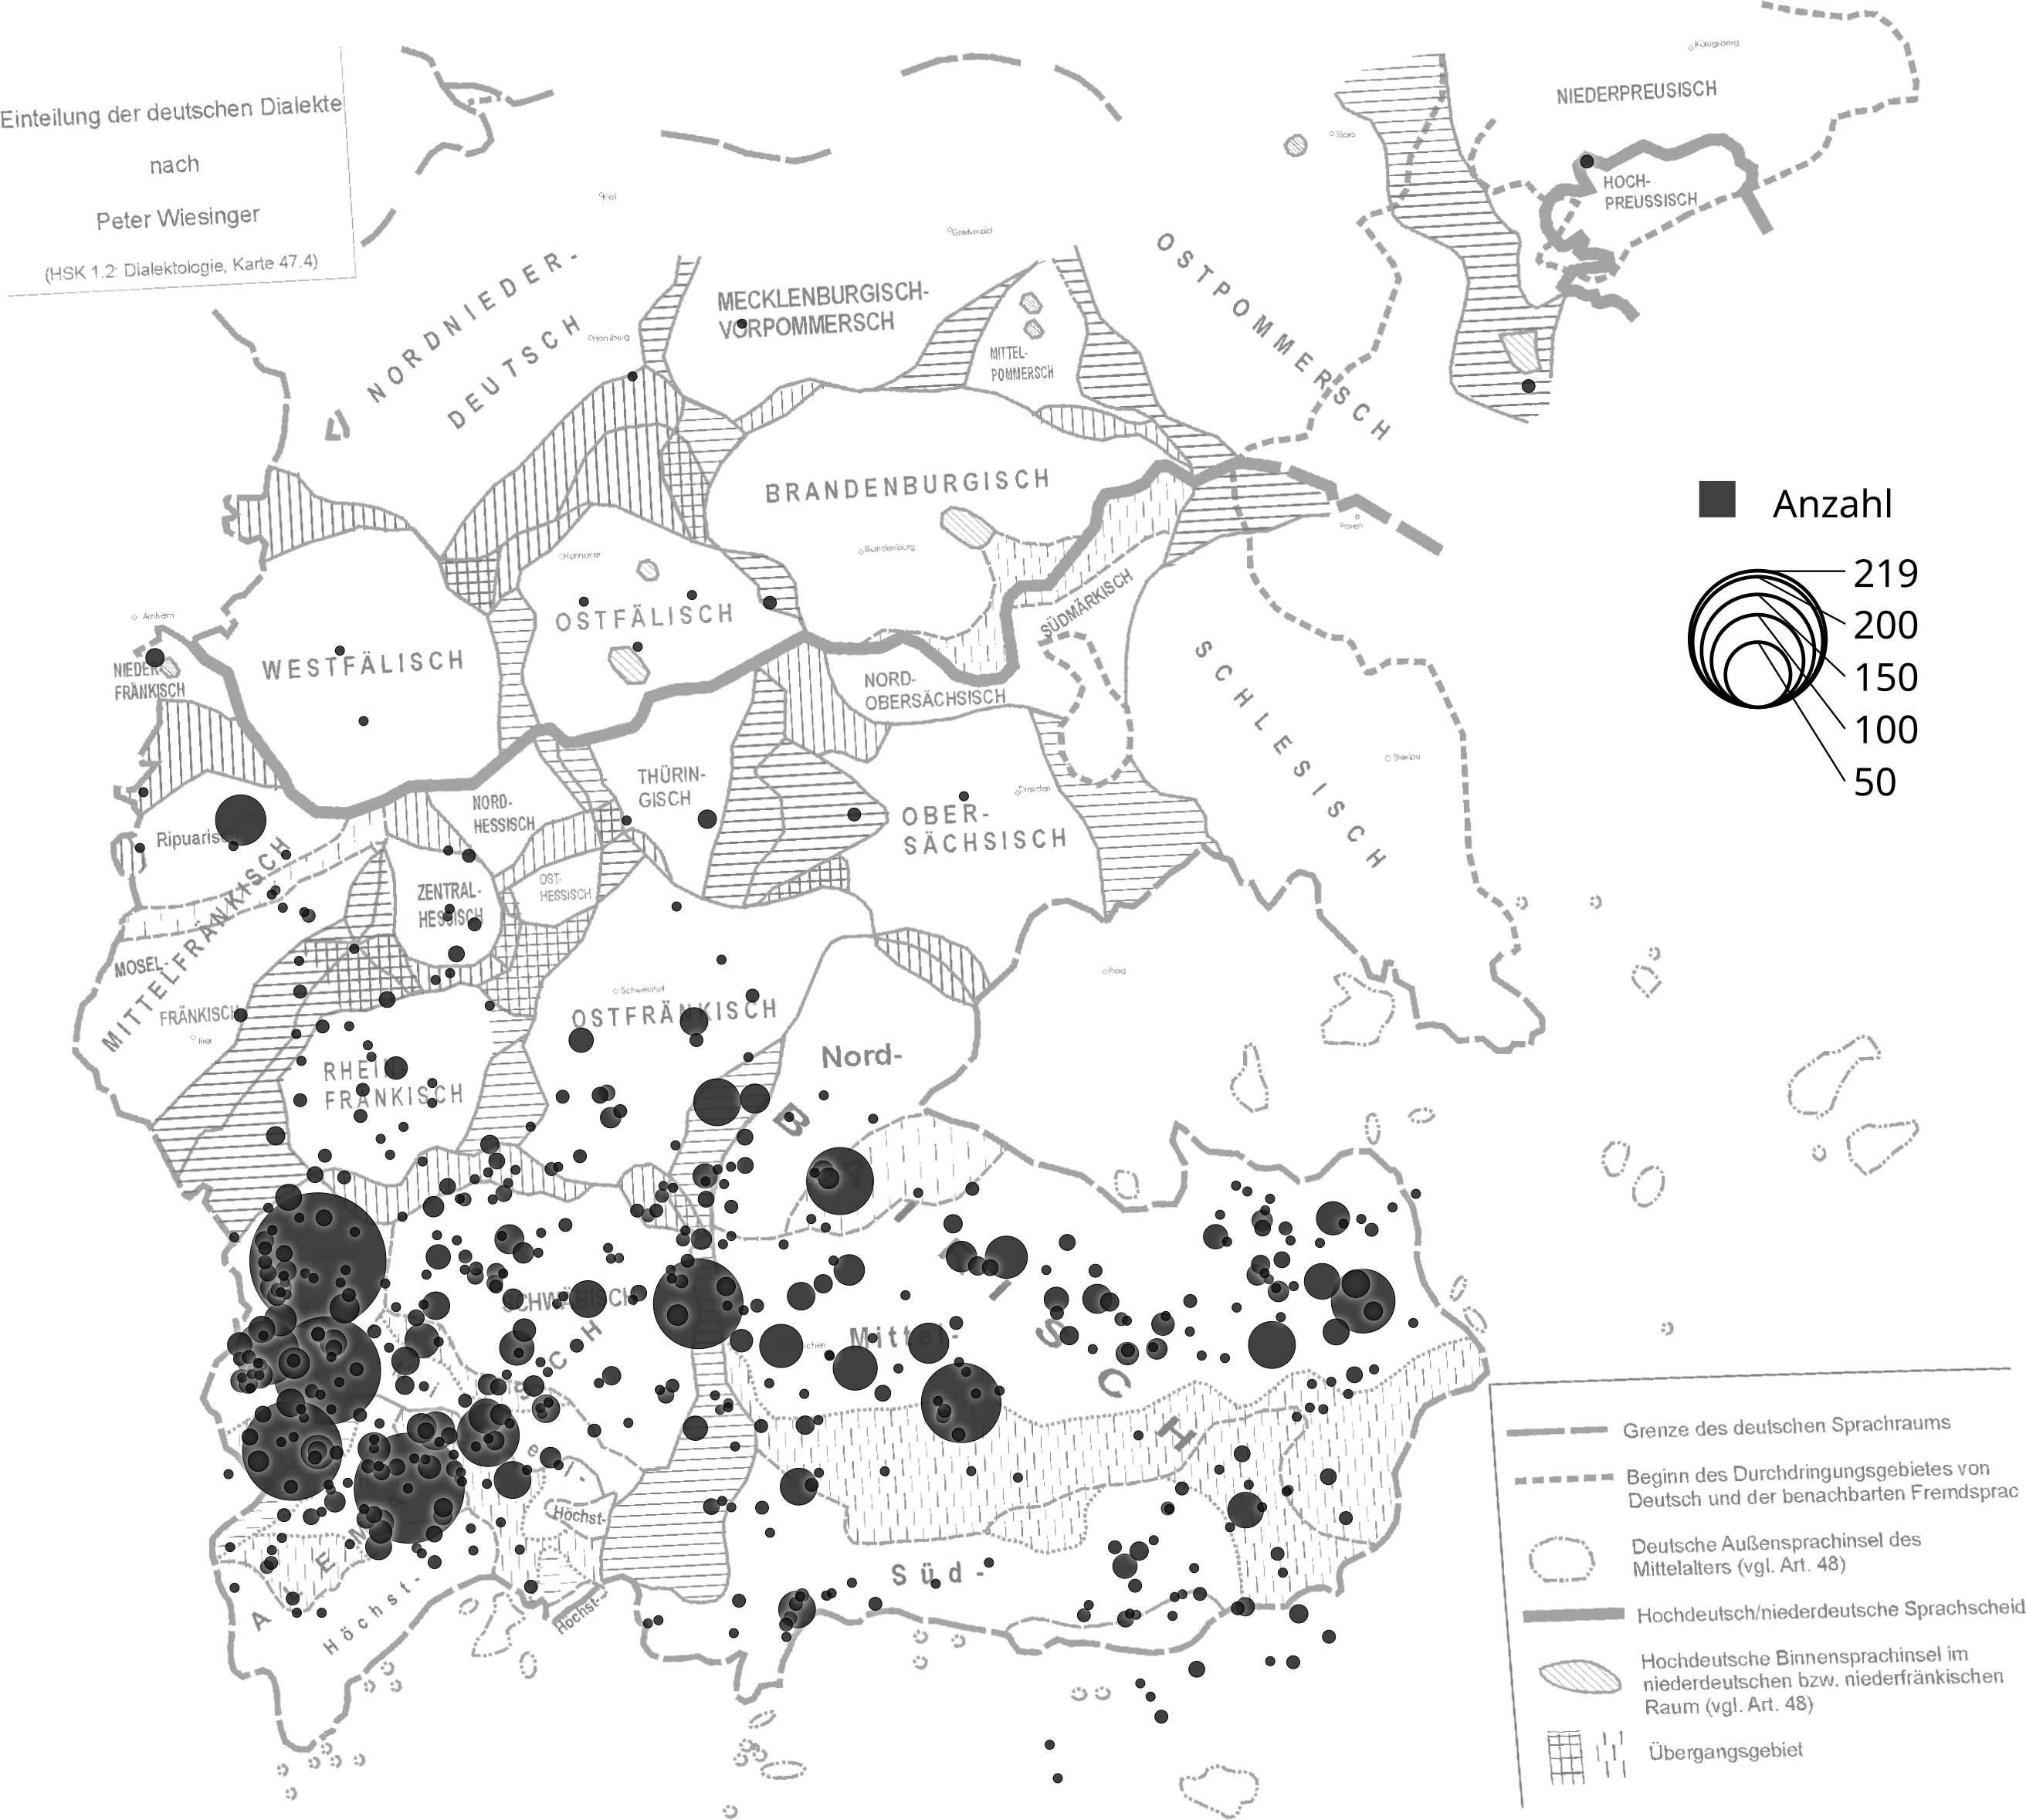
\includegraphics[
	width=\linewidth,
	height=.95\textheight,
	keepaspectratio
]{./assets/grafiken/2022-03-03_deedsperplace.png}
\caption%
	[Urkunden pro eindeutigem \citetitle{cao}-Ausstellungsort]%
	{Urkunden pro eindeutigem \citetitle{cao}-Ausstellungsort}
\label{fig:cao_urkorte}
\end{figure}
\end{landscape}%
}

Das \citetitle{cao} hat den Anspruch, die gesamte Urkundenüberlieferung des
13.~Jahrhunderts zu versammeln. Auch wenn es eine \q*{Dunkelziffer} an Urkunden
gibt, die nicht in die Sammlung aufgenommen wurden, wird die Zunahme an
deutschsprachigen Urkunden in \cref{tab:urkstat} deutlich; der Großteil der
Urkunden im \citetitle{cao} entfällt auf die letzten beiden Jahrzehnte. Während
der westoberdeutsche Sprachraum zunächst bei der Ausstellung deutschsprachiger
Urkunden führt, holt der ostoberdeutsche ab den 1280er Jahren massiv auf und
übertrifft den westoberdeutschen am Ende der Dekade schließlich um etwa
4,6\pct{} \autocite[46--47]{ganslmayer2012}.%
%
	\footnote{\citet[47]{ganslmayer2012} weist im Abschnitt von 1290--1299 für
		das Alemannisch-Schwäbische 38,79\pct{} der im \citetitle{cao}
		enthaltenen Urkunden aus sowie für das Bairische insgesamt 43,4\pct.
	}

\begin{table}
\centering
\caption{Anzahl der Urkunden im \citetitle{cao} pro Jahrzehnt
\autocite[40]{ganslmayer2012}}
\begin{tabularx}{\textwidth}{l C C C C}
\toprule
%
	& \textbf{bis 1279}
	& \textbf{1280--1289}
	& \textbf{1290--1299}
	& \textbf{Summe}
	\\

\midrule

Anzahl insgesamt
	& 621
	& 1.095
	& 2.901
	& 4.617
	\\

\midrule

davon deutschsprachig
	& 585
	& 1.007
	& 2.697
	& 4.289
	\\

\bottomrule
\end{tabularx}
\label{tab:urkstat}
\end{table}

Insgesamt lässt sich festhalten, dass die Urkunden des \citetitle{cao} für
linguistische Fragestellungen eine Reihe von Vorteilen bieten. Zum einen
handelt es sich um Gebrauchsprosa, die im Rahmen von großteils privaten
Rechtsgeschäften das alltägliche Leben der Zeit in vielfältiger Weise berühren.
Damit stehen die Urkundentexte tendenziell näher an der Alltagssprache als
literarische Texte, die besonders in der älteren Grammatikschreibung zum
Mittelhochdeutschen überproportional repräsentiert waren. Die Urkunden stellen
in der Regel das schriftlich festgehaltene Ergebnis mündlich geführter
Verhandlungen dar \autocite[595]{schmidtwiegand1998b}. Zum anderen ist das
\citetitle{cao} für sprachgeschichtliche Untersuchungen gut geeignet, da
größter Wert auf eine zuverlässige Transkription gelegt wurde. Die Urkunden
sind darüber hinaus zumeist datiert und enthalten Informationen, mit denen sie
sich regional zuordnen lassen, was gerade für sprachgeografisch orientierte
Analysen eine ideale Voraussetzung ist \autocite[22]{schulze2011}.

Obwohl bei der vorliegenen Untersuchung nicht sämtliche Urkunden untersucht
wurden (vgl. \cref{sec:miningcao}), ist das Ortsnetz dicht genug, dass
Raumstrukturen zutage treten. Besonders hervorzuheben ist der Umstand, dass das
insgesamt zirka zwei Millionen Wortformen umfassende Textkorpus (das heißt
einschließlich der Mehrfachausfertigungen und nicht-deutschsprachiger Urkunden)
vollständig elektronisch vorliegt \autocites{gniffkerapp2005}{cao-online} und
damit eine ansehnliche Datenmenge in ihrer ganzen Breite handhabbar wird
\autocite{beckerschallert2021,beckerschallert2022b}.%
%
	\footnote{Zum Vergleich mit anderen elektronischen Korpora zu historischen
	Sprachstufen des Deutschen siehe \citet{dipper2015}.
	\citet[391]{gniffkerapp2005} beziffern den Umfang des \citetitle{cao} mit
	\blockquote{etwa 1,3 Millionen Belegwörtern}, wobei sie sich dabei
	vermutlich nur auf das deutschsprachige Material ohne Doppelausfertigungen
	beziehen.} % (vgl.~\cref{fn:caowordcount}).}

Nachteilig ist, dass nicht an jedem Ort gleich große Mengen an Urkunden
vorliegen, zumal die Urkunden des \citetitle{cao} lediglich eine Momentaufnahme
größtenteils der letzten zwanzig Jahre des 13.~Jahrhunderts bieten. Darüber
hinaus besteht das Problem, dass sich Schreiberinnen und Schreiber in der Regel
nicht greifen lassen, sodass aus der einzelnen Urkunde heraus nicht deutlich
wird, ob sie genuin ortstypische Sprache reflektiert. Diesen Nachteilen lässt
sich jedoch mit einer Kombination von quantitativer und qualitativer Analyse
begegnen. Da einzelne Belege wenig aussagen, braucht es eine gewisse Masse an
Belegen, um Tendenzen deutlich zu machen.
% Andererseits ist es informativ, das Spezifische an abweichenden Einzelbelegen
% in Relation zum Gesamtbild zu setzen.
Zu kleinteiligen Aus\-sagen zur Mundart einzelner Orte wird man über die
Untersuchung der Urkunden nicht gelangen, wohl aber zu Aussagen über das
Verhalten unterschiedlicher Schreibregionen und die Reflexion divergierender
Sprachmerkmale im regionalen Schreibgebrauch.

%%%%%%%%%%%%%%%%%%%%%%%%%%%%%%%%%%%%%%%%%%%%%%%%%%%%%%%%%%%%%%%%%%%%%%%%%%%%%%%

\section[Die \tit{Kaiserchronik}]{Die \citetitle{kc}}
\label{sec:materialkc}

Die \citetitle{kc} ist eine Reimchronik in deutscher Sprache, die um die Mitte
des 12.~Jahrhunderts vermutlich in Regensburg entstanden ist.%
%
	\footnote{Einen Überblick bietet \citet{nellmann1983}. Zum aktuellen
	Forschungs- und Editionsstand siehe das ZfdA-Themenheft zur \citet{kc}
	\autocite{wolf2019} sowie jüngst die Dissertation von \citet{weis2022}.
	Angaben zur Entstehungszeit und zum Schreibdialekt der jeweiligen
	Textzeugen basieren auf dem derzeit noch unveröffentlichten Katalog von
	\citet{wolf:kckat}, siehe auch \urlcite{kcdigital}\nocite{kcdigital}
	sowie den \citet[s.\,v.~\textit{\tit{Kaiserchronik}}]{hsc} mit den dort
	angegebenen Quellen.}
%
Sie ist anonym überliefert und auch die Frage nach ihrem Auftraggeber ist
ungeklärt. \citet[92]{wolf2008} bescheinigt der \citet{kc}
\blockquote{ein Formen-, Sprach- und Normeninventar, das für die
volkssprachig-höfische Literatur des Spätmittelalters zu einem Grundmuster
wird}.

Der Text ist in bislang fünfzig bekannten Textzeugen zwischen dem letzten
Viertel des 12.~Jahrhunderts \autocites{kc:A1} und dem späten 16.~Jahrhundert
\autocite{kc:T} überliefert \autocite[39, 57]{wolf:kckat}; der
Überlieferungsschwerpunkt fällt in das 13.~Jahrhundert
\autocites[vgl.][s.\,v.~\textit{\tit{Kaiserchronik}}]{hsc}{kcdigital}. Im Lauf
ihrer etwa vierhundertjährigen Überlieferungsgeschichte hat die \citet{kc} zwei
Überarbeitungen erfahren: um ca.~1200 (\q*{Rezension~B}) und um ca.~1250
(\q*{Rezension~C}) \autocites%
% [367--368]{gaertner1995}
{wolf2008}.
% [142]{chincaetal2019a}.
\citet[369]{gaertner1995} zufolge unterscheiden sich die Rezensionen B und C so
stark von der ältesten Fassung (\q*{Rezension~A}), dass sie jeweils neue Werke
darstellen; \citet[142]{chincaetal2019a} sprechen mit \citet{bumkepeters2005b}
in diesem Zusammenhang von \q*{Retextualisierung}.

% \afterpage{
% \begin{landscape}
% % \begin{vplace}
% \vfill
% \begin{figure}
% \centering
% \subfloat[{%
% 		\citelist{kc:A1}{location},
% 		\citefield{kc:A1}{library},
% 		\citefield{kc:A1}{shelfmark}
% 		\autocites*(\cite[1432]{hsc})[\pno~1\ro]{kc:A1}
% 	}]{
% 	\includegraphics[
% 		width=.32\linewidth,
% 	]{./assets/grafiken/Vorau-StAV-Ms276-001r.jpg}
% }
% \hfill
% \subfloat[{%
% 		\citelist{kc:B1}{location},
% 		\citefield{kc:B1}{library},
% 		\citefield{kc:B1}{shelfmark}
% 		\autocites*(\cite[2693]{hsc})[\pno~2\vo]{kc:B1}
% 	}]{
% 	\includegraphics[
% 		width=.32\linewidth,
% 	]{./assets/grafiken/Wien-OeNB-Cod2779-002v.jpg}
% }
% \hfill
% \subfloat[{%
% 		\citelist{kc:C1}{location},
% 		\citefield{kc:C1}{library},
% 		\citefield{kc:C1}{shelfmark}
% 		\autocites*(\cite[2013]{hsc})[\pno~1\ro]{kc:C1}
% 	}]{
% 	\includegraphics[
% 		width=.32\linewidth,
% 	]{./assets/grafiken/Wien-OeNB-Cod2685-001r.jpg}
% }
% \caption%
% 	[Die Textanfänge der drei Leithandschriften des Editionsprojekts zur
% 	\tit{Kaiserchronik}]%
% 	{Die Textanfänge der drei Leithandschriften des Editionsprojekts zur
% 	\citet{kc} von \citeauthor{chincaetal2019b}}
% \label{fig:kcincipits}
% \end{figure}
% \vfill
% % \end{vplace}
% \end{landscape}
% }

Die \citet{kc} handelt ihrer eigenen Aussage nach
\norm{von den bâbesen unt von den chunigen, baidiu guoten unt ubelen}
\wdef{von den Päpsten und von den Königen, sowohl guten als auch schlechten}
\autocite[19--20]{schroeder1895}. Die einzelnen Episoden zu den jeweiligen
Kaisern von Cäsar bis Konrad~III.\ (A/B), beziehungsweise je nach Fortsetzung
Friedrich~II. oder Rudolf~I. (C), verselbstständigen sich bisweilen zu eigenen
Erzählungen und haben eher den Charakter eines Fürstenspiegels als den eines
strikt historiografischen Abrisses, zumal die historische Reihenfolge der
Kaiser nicht immer eingehalten wird, zwei römische Kaiser hinzugedichtet werden
und die Angaben zu den Regierungszeiten der jeweiligen Kaiser am Ende jeder
Episode willkürlich sind \autocite[954--960]{nellmann1983}. Stattdessen soll
\blockcquote[957]{nellmann1983}{\textins*{m}öglichst jede Kaisergeschichte
\textelp{} den \textquote{heilsgeschichtlichen Kampf der guten und der bösen
Mächte} \textelp{}
% (\textsc{Ohly}, S. 238)
% (\textsc{\citeauthor{ohly1968}}, \notecite[\pno~238]{ohly1968})
% \textins{\cite[238]{ohly1968}}
zur Anschauung bringen}.

Erste Ausgaben des Volltexts der \citet{kc} erfolgten von \citet{massmann:kukb}
sowie von \citet{diemer1849} nach der damals gerade neu entdeckten Vorauer
Handschrift \citep{kc:A1}. Die bisher maßgebliche Edition ist die von
\nosh\citet{schroeder1895}. Die genannten drei Editionen geben alle den Text
der Rezension~A wieder, \citeauthor{massmann:kukb} bietet ausschnittsweise auch
Teile von B und C.%
%
	\footnote{Ein kritisches Resümee zur Editionstätigkeit
		\citeauthor{massmann:kukb}s zieht \citet{wolf2023}, in Bezug auf die
		\textcite{kc} siehe dort, \notecite[\pno~122--132]{wolf2023}.
		\citeauthor{massmann:kukb}s Edition der \textcite{kc} beruht auf der
		Heidelberger A-Handschrift (\citet{kc:H}), deren Text er mäßig
		normalisiert im Grunde als Leithandschrift bietet, allerdings ermangelt
		sein Text bisweilen philologischer Stringenz und ist damit nicht
		unproblematisch \autocite[125--126]{wolf2023}. Obwohl
		\citeauthor{massmann:kukb} nach \posscite[131--132]{wolf2023} Urteil
		zugute zu halten ist, dass in den \textquote{Beigabenpaketen} auch zur
		\textcite{kc}-Edition durchaus viel Nützliches an Meta-, Inter- und
		Paralleltexten enthalten ist, zeichnen sich diese Beigaben durch
		\textquote{eine überbordende Fülle gepaart mit einer chaotisch
		anmutenden Un-Ordnung} negativ aus, \textcquote[131]{wolf2023}{und zwar
		insbesondere dann, wenn Fakten und Phantasie (bei Maßmann nicht selten)
		zusammenfließen}, vor allem im Sinne seiner vom Nationalismus geprägten
		politisch-historischen Interessen.%
	}
%
Die Edition von \citeauthor{schroeder1895} ist zwar normalisiert, insofern
Schreibweisen vereinheitlicht sowie Vokallängen und moderne Interpunktion
eingefügt wurden. Sie verfolgt im Großen und Ganzen aber das
Leit\-handschriften\-prinzip auf der Grundlage von \citet{kc:A1}.
\citeauthor{diemer1849} stellt einen diplomatischen Abdruck zur Verfügung. Eine
textkritische Ausgabe, die die Texte der Rezensionen~B und C als
gleichberechtigt neben A behandelt, ist bisher ein Desiderat.

Mit dem Projekt zur Neuedition der \citet{kc} in Form einer synoptischen
Ausgabe wird die Einlösung dieses Desiderats unter der Leitung von Mark Chinca,
Helen Hunter, Christopher Young (Cambridge) und Jürgen Wolf (Marburg) seit 2012
verfolgt \autocite{chincaetal2019b}. Zu diesem Zweck wurden sämtliche bekannten
und noch existenten Textzeugen auf Basis von Digitalfotos der
Handschriften\-originale diplomatisch transkribiert. Farb\-digitalisate und
XML-kodierte Transkriptionen sind über die Universität Heidelberg öffentlich
zugänglich.%
%
	\footnote{Siehe \urlcite{kcdigital}\nocite{kcdigital}.}
%
% Wenn die \citet{kc} hier als Untersuchungs\-gegenstand dient, dann nicht in
% Hinsicht auf eine literaturwissenschaftliche Fragestellung oder unter
% editionsphilologischen Aspekten, sondern unter denen der historischen
% Sprachwissenschaft.
\citet[287]{chincaetal2019b} betonen, dass mit der digitalen Edition der
\citetitle{kc} \blockquote{Sprachhistoriker \textelp{}
die Möglichkeit \textins*{haben}, Vorgänge der dia\-topischen und
dia\-chronischen Mikrovarianz zu beobachten, die im textkritischen Apparat
normalen Formats sonst verlorengingen}.

Die einzelnen Textzeugen sind regional verhältnismäßig breit gestreut, haben
allerdings ihren Überlieferungsschwerpunkt im Ostoberdeutschen, wie
\cref{fig:kc_geospac_rough} deutlich macht
(\cite[vgl.~auch][]{klein1988} für die Rezension~A).%
%
	\footnote{Anders als bei den Urkunden kann für die jeweiligen
		\citet{kc}-Textzeugen in der Regel kein mehr oder weniger exakter
		Entstehungsort ermittelt werden, daher dienen die Markierungen auf der
		Karte lediglich der Übersicht. Maßgeblich als Angaben zur
		sprachräumlichen Einordnung sind die Beschriftungen
		\autocite[vgl.][]{wolf:kckat}.}
%
Ähnlich wie bei den Urkunden des \citetitle{cao} liegt eine Textsammlung
sozusagen \q*{aus einem Guss} vor, da alle enthaltenen Texte dem gleichen
literarischen Werk zugeordnet sind. Ein fundamentaler Unterschied zu den
Urkunden liegt in der Art und Weise der Tradierung des Großteils
mittelalterlicher Texte: \blockquote[{\cites[1310]{wegera2000}[siehe
auch][262--263]{fleischer2019}}]{In der Regel haben wir es mit einer längeren
Text- und Rezeptionsgeschichte, also mit Abschriften und Abschriften von
Abschriften zu tun. Es muß deshalb mit einer erheblichen regional bedingten
Interferenz und mit einer zeitlichen Verzerrung des Sprachstandes gerechnet
werden (Stichwort: Vorlagenproblematik).}

\afterpage{%
\begin{landscape}
\begin{figure}
\centering
\subfloat[12.~Jahrhundert]{
	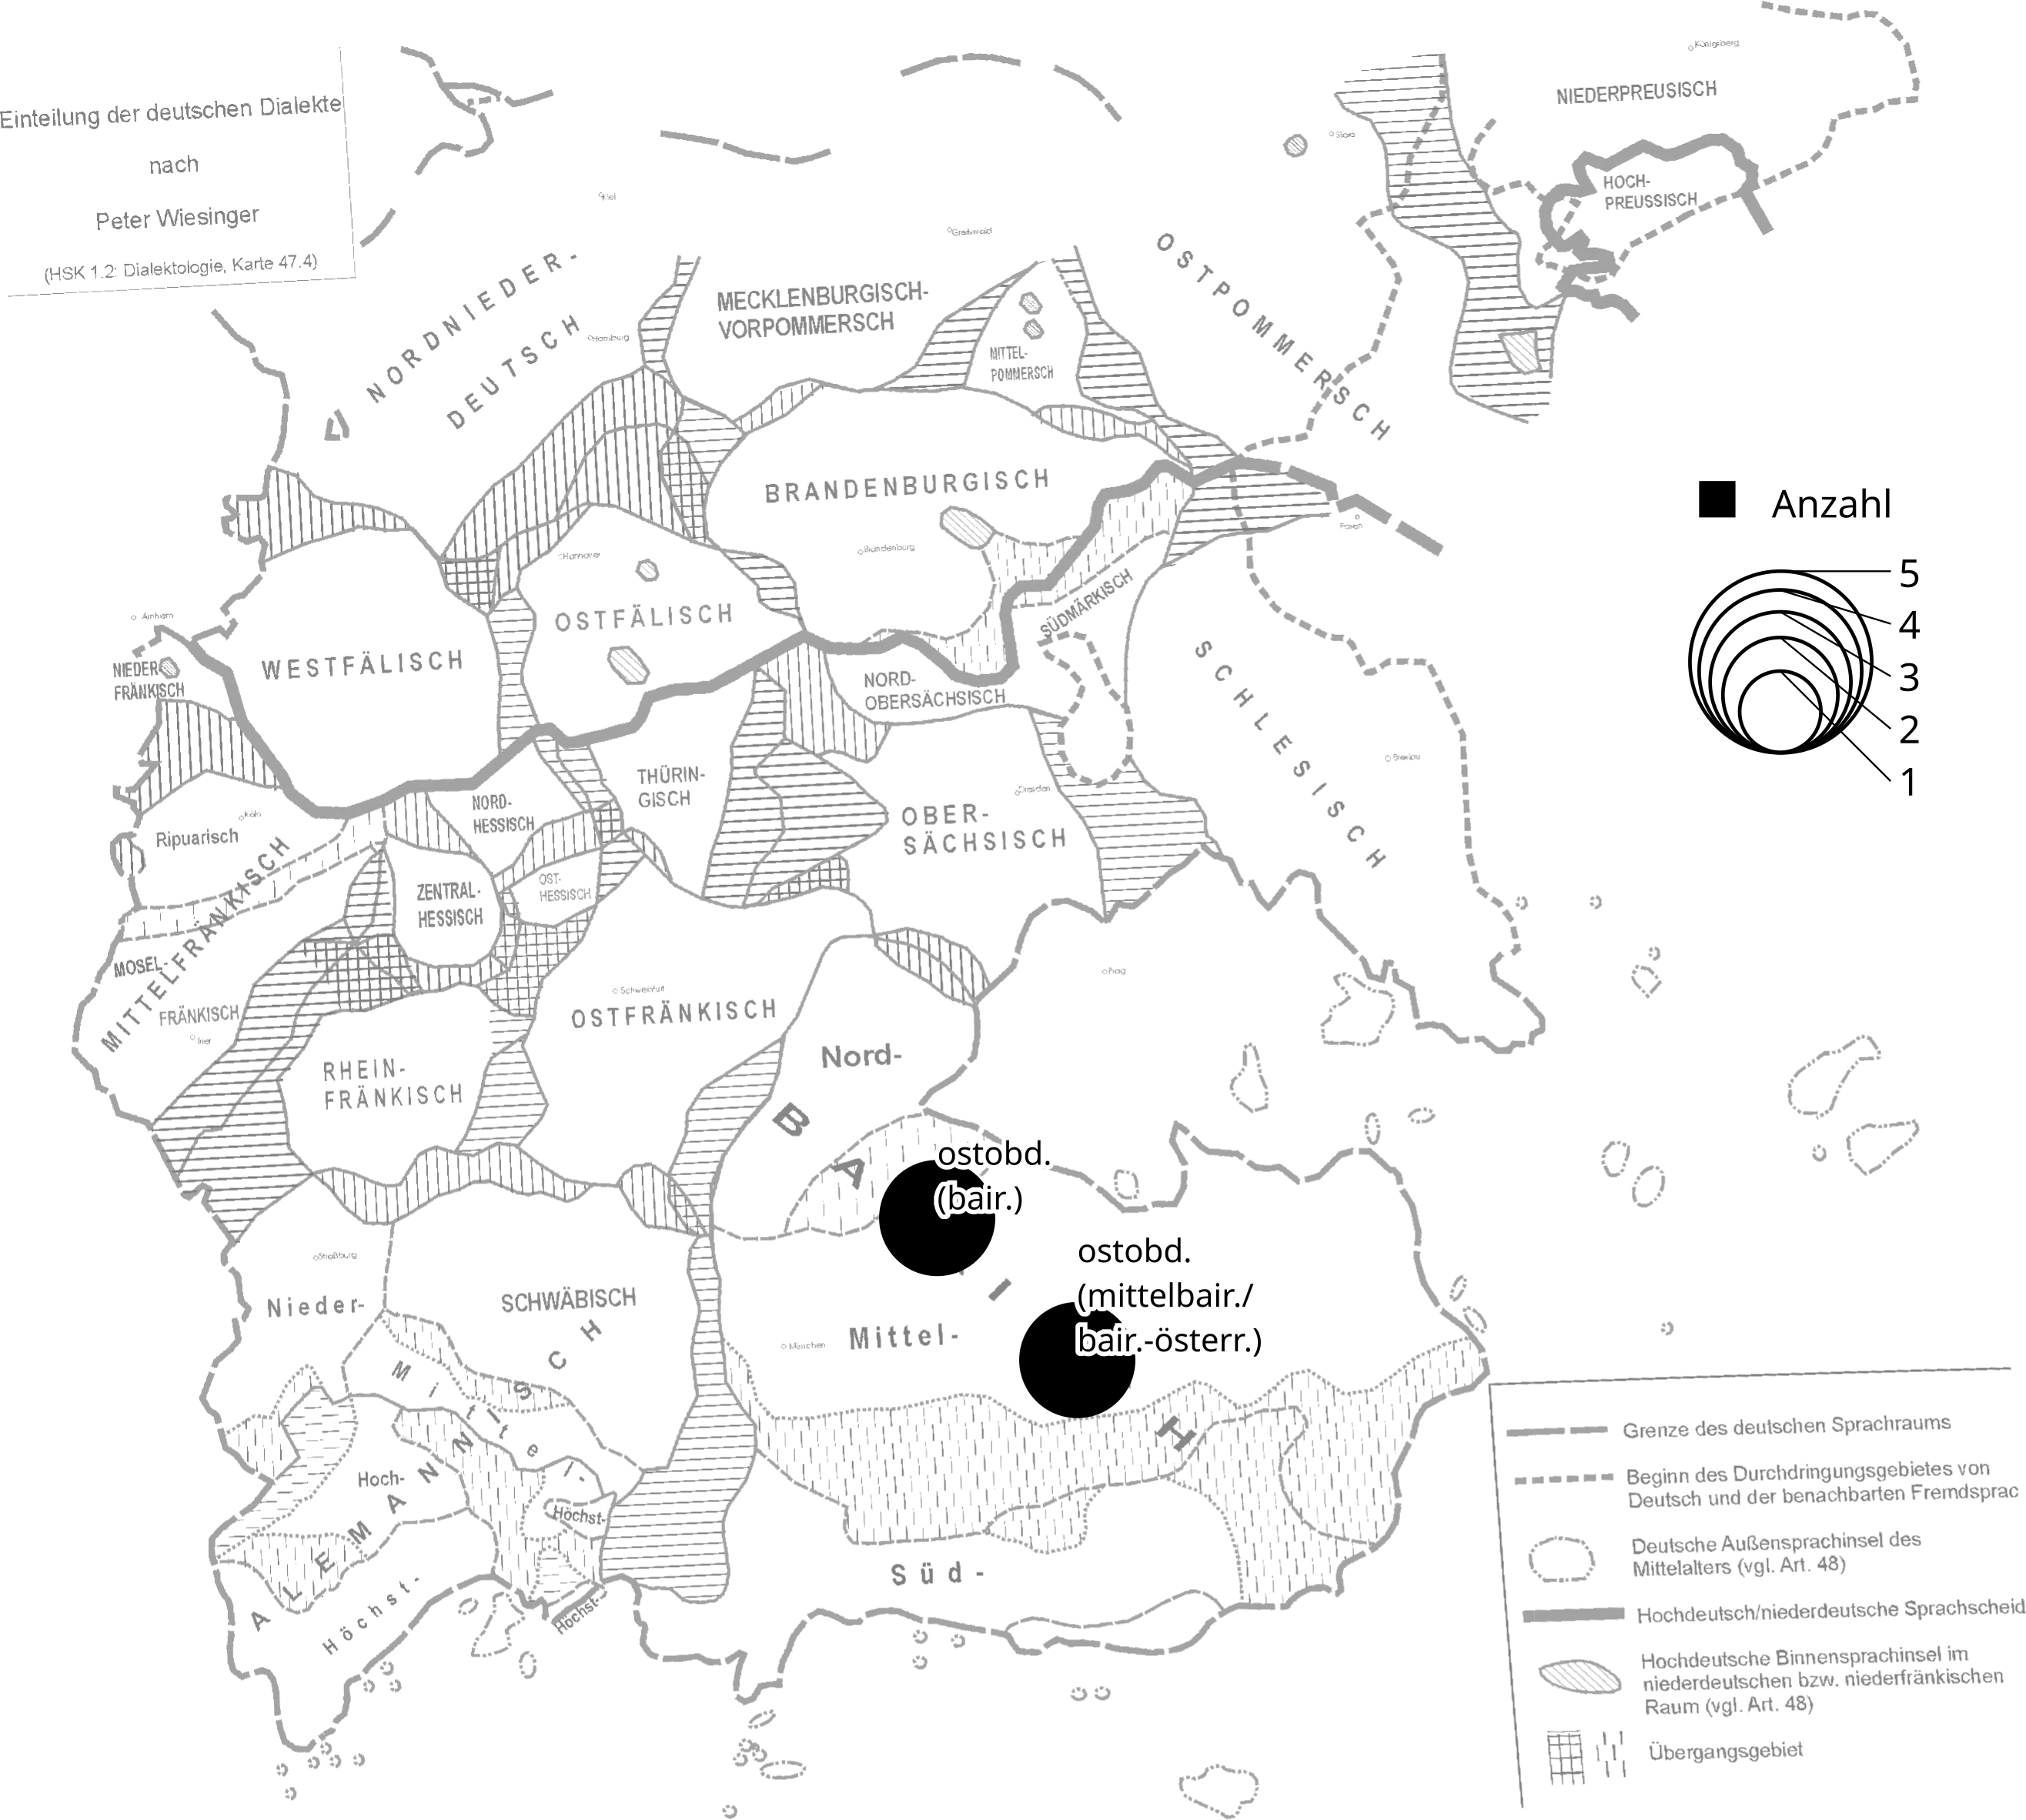
\includegraphics[
		width=.49\linewidth,
		height=.95\textheight,
		keepaspectratio
	]{./assets/grafiken/2021-12-30_kc_geospac_rough_c12.png}
}
\subfloat[13.~Jahrhundert]{
	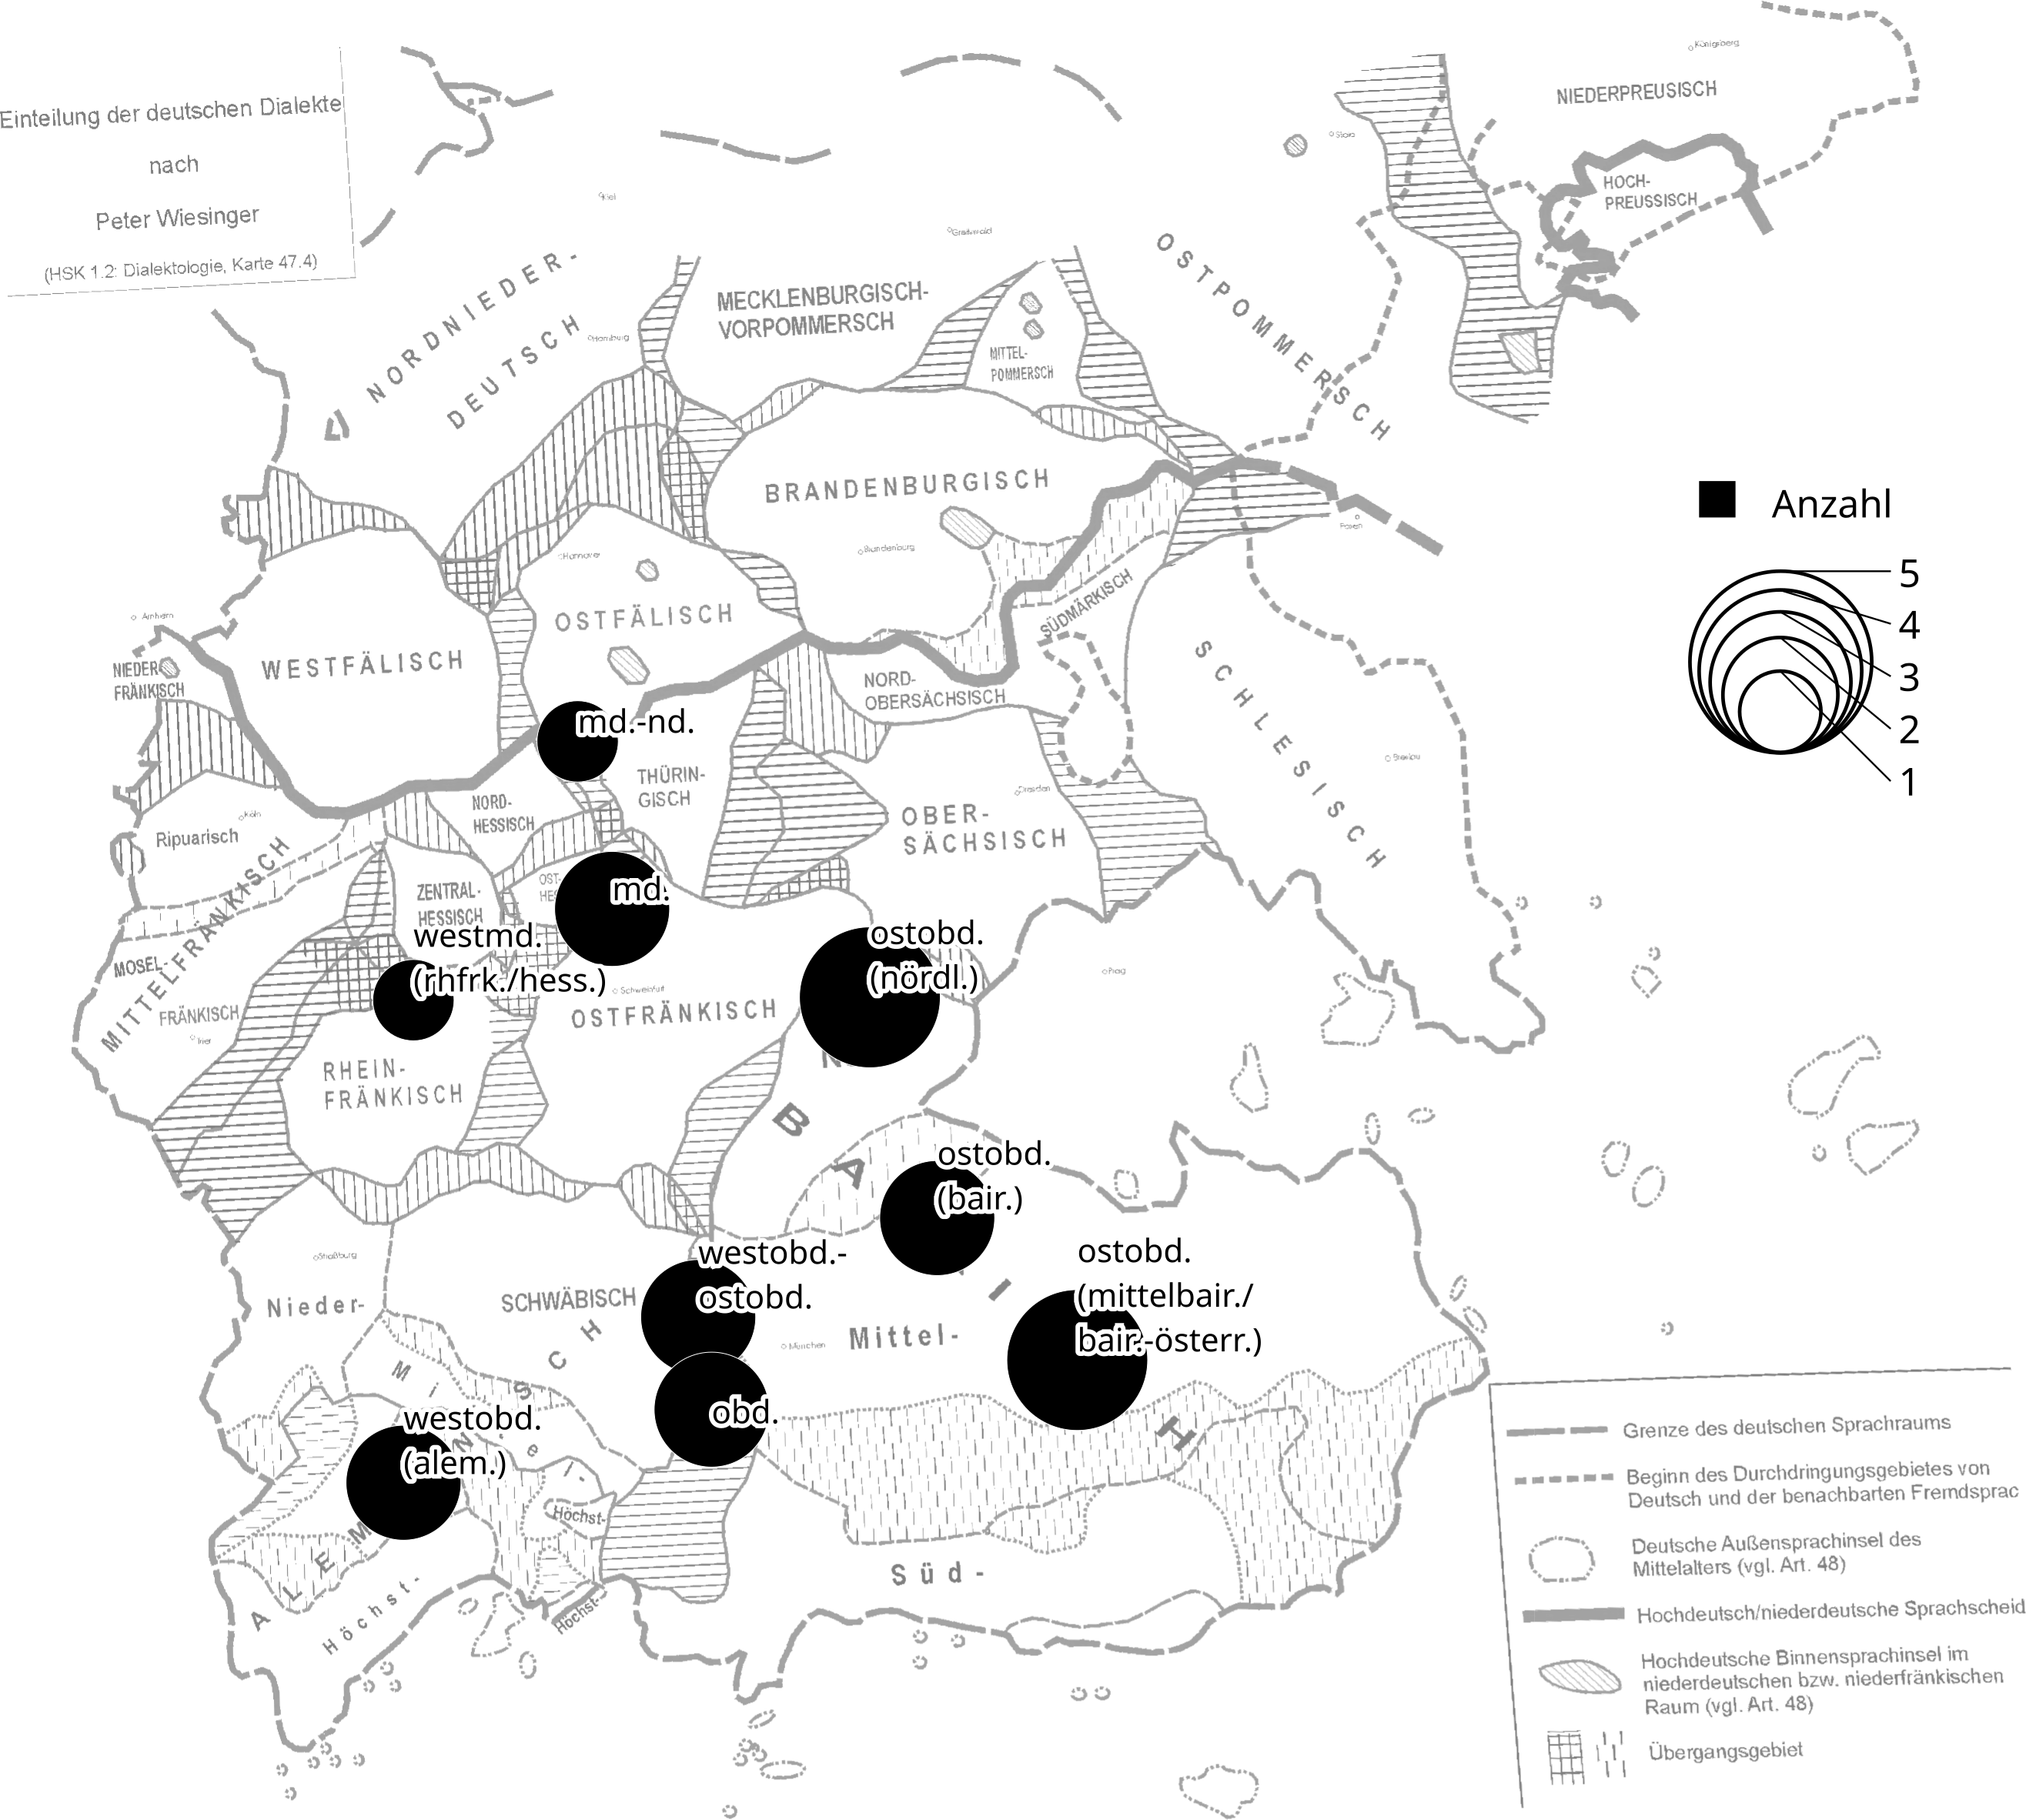
\includegraphics[
		width=.49\linewidth,
		height=.95\textheight,
		keepaspectratio
	]{./assets/grafiken/2021-12-30_kc_geospac_rough_c13.png}
}
\caption%
	[Grobe räumliche und zeitliche Verteilung der \citet{kc}-Textzeugen]%
	{Grobe räumliche und zeitliche Verteilung der \citet{kc}-Textzeugen
		\nocite{wiesinger1983:rede}
	}
	\label{fig:kc_geospac_rough}
\end{figure}

\begin{figure}
\ContinuedFloat
\subfloat[14.~Jahrhundert]{
	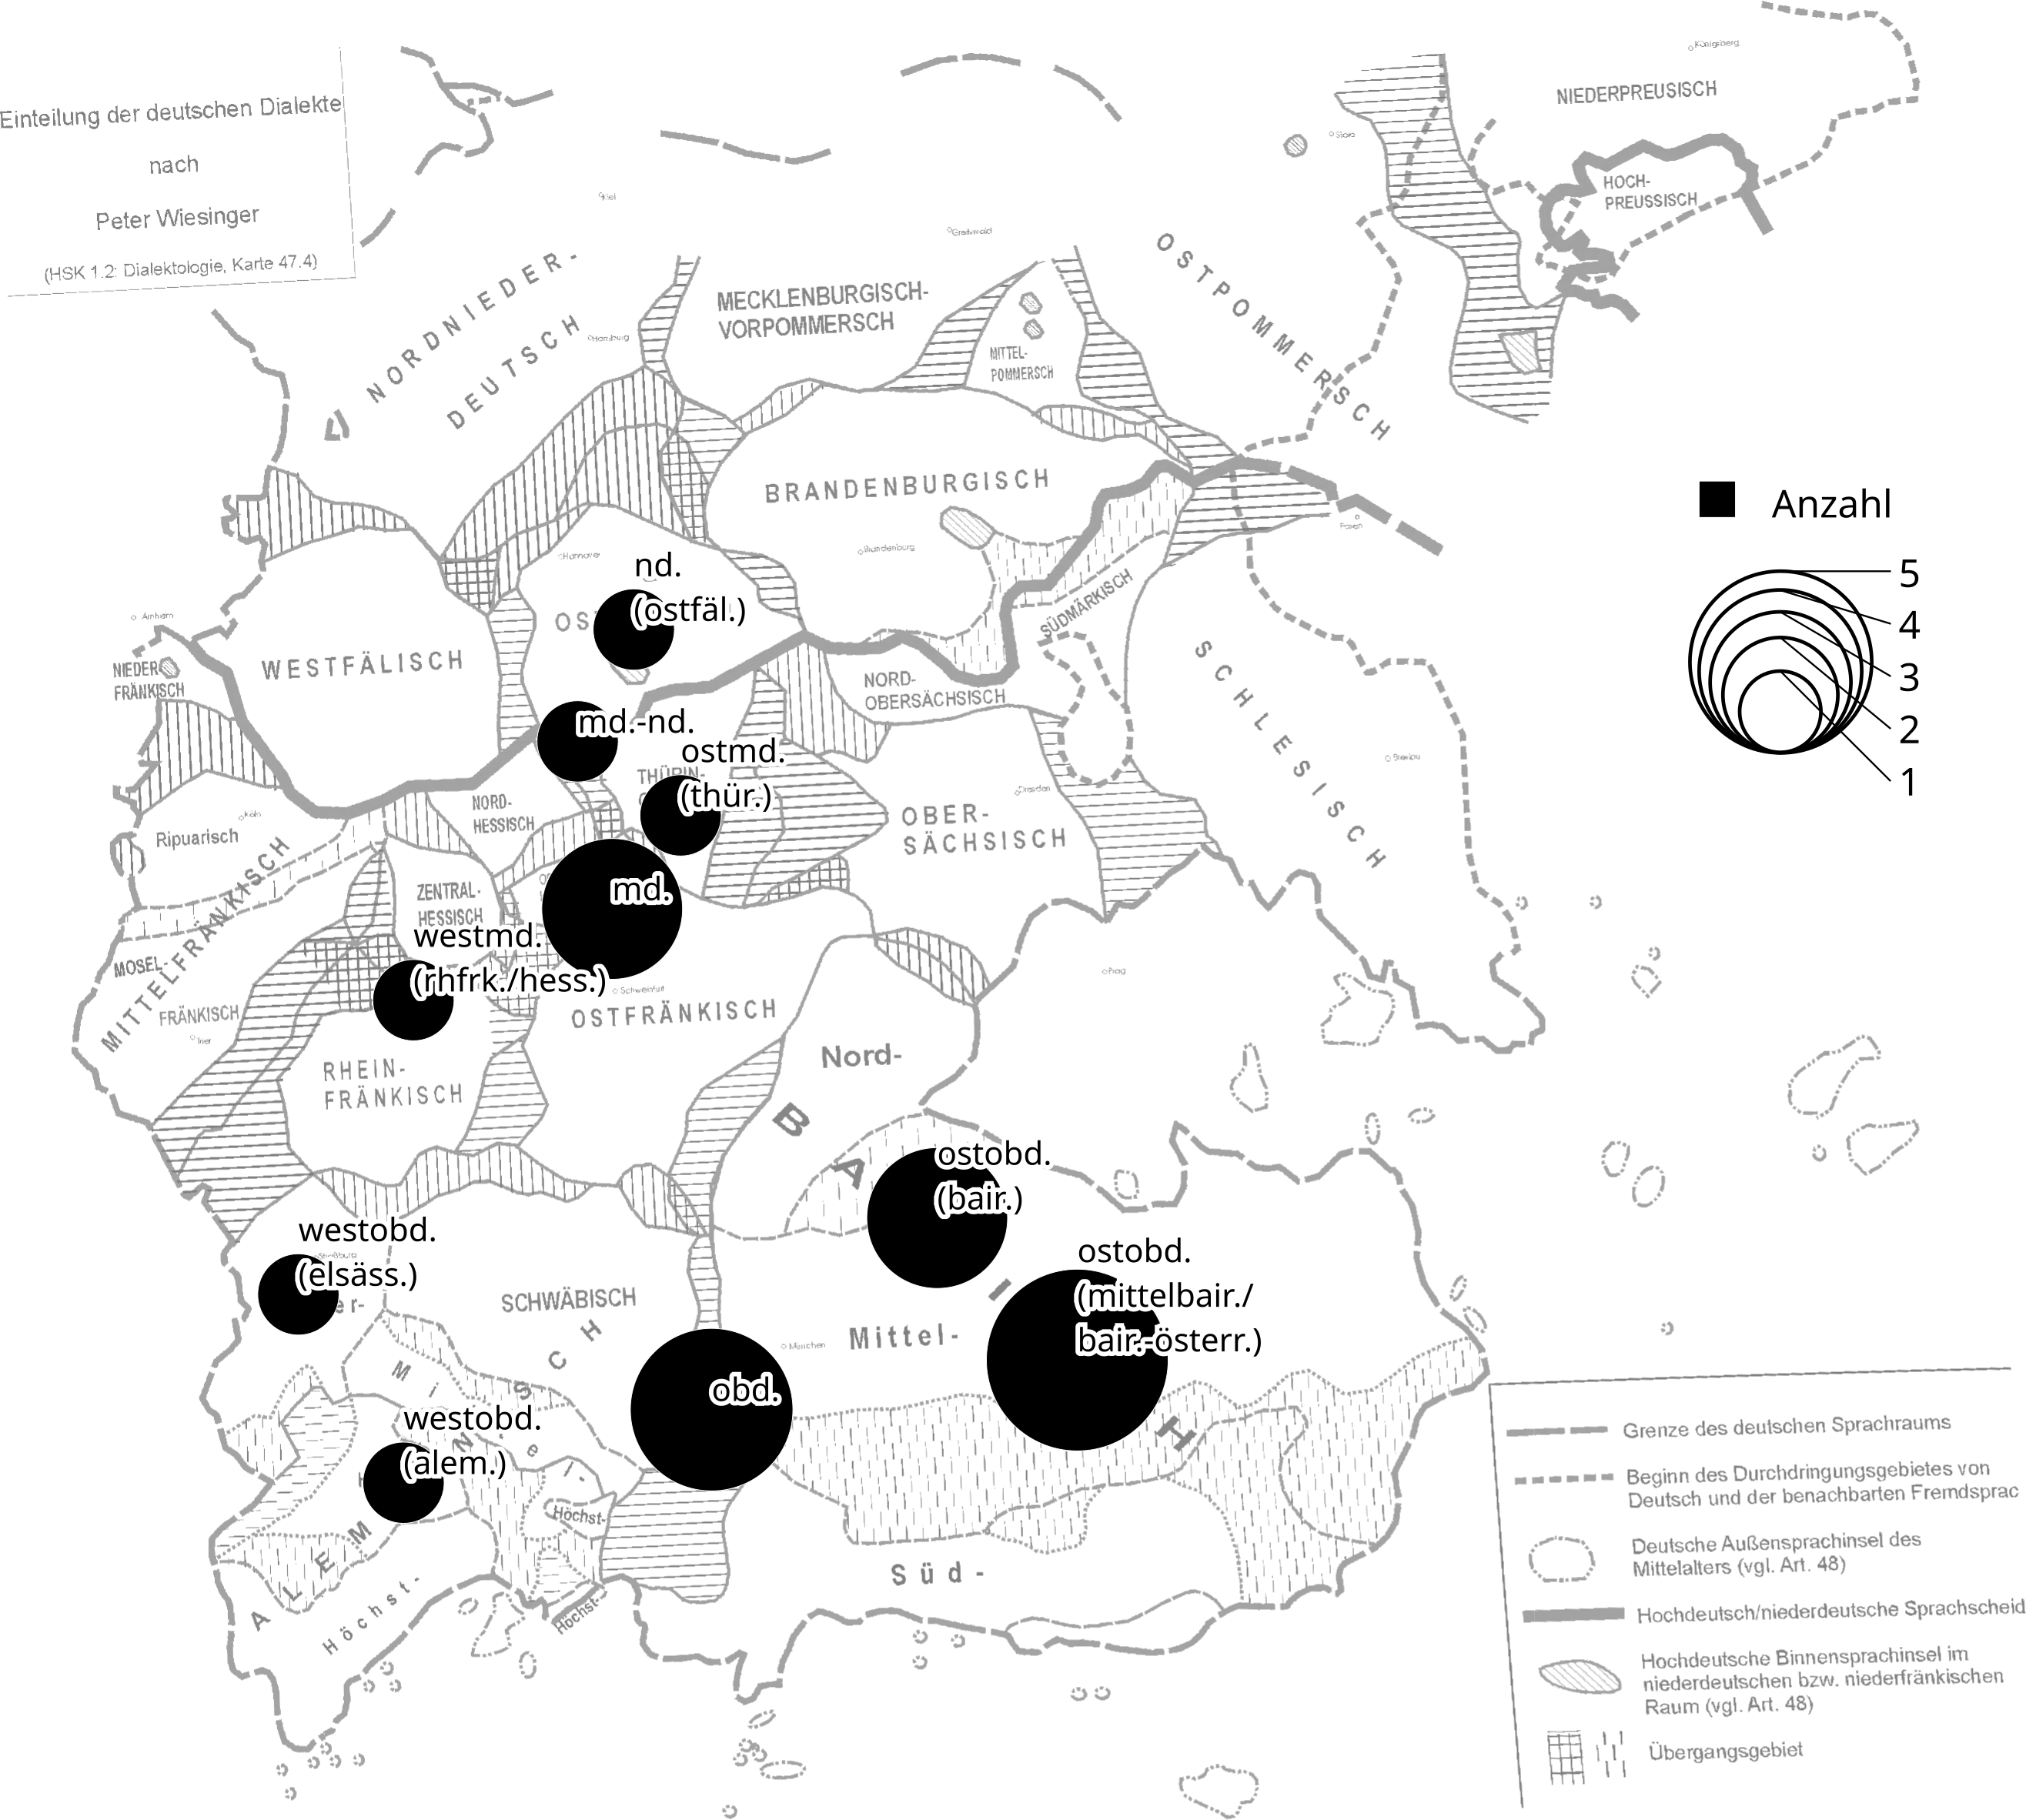
\includegraphics[
		width=.49\linewidth,
		height=.95\textheight,
		keepaspectratio
	]{./assets/grafiken/2021-12-30_kc_geospac_rough_c14.png}
}
\subfloat[15.~Jahrhundert]{
	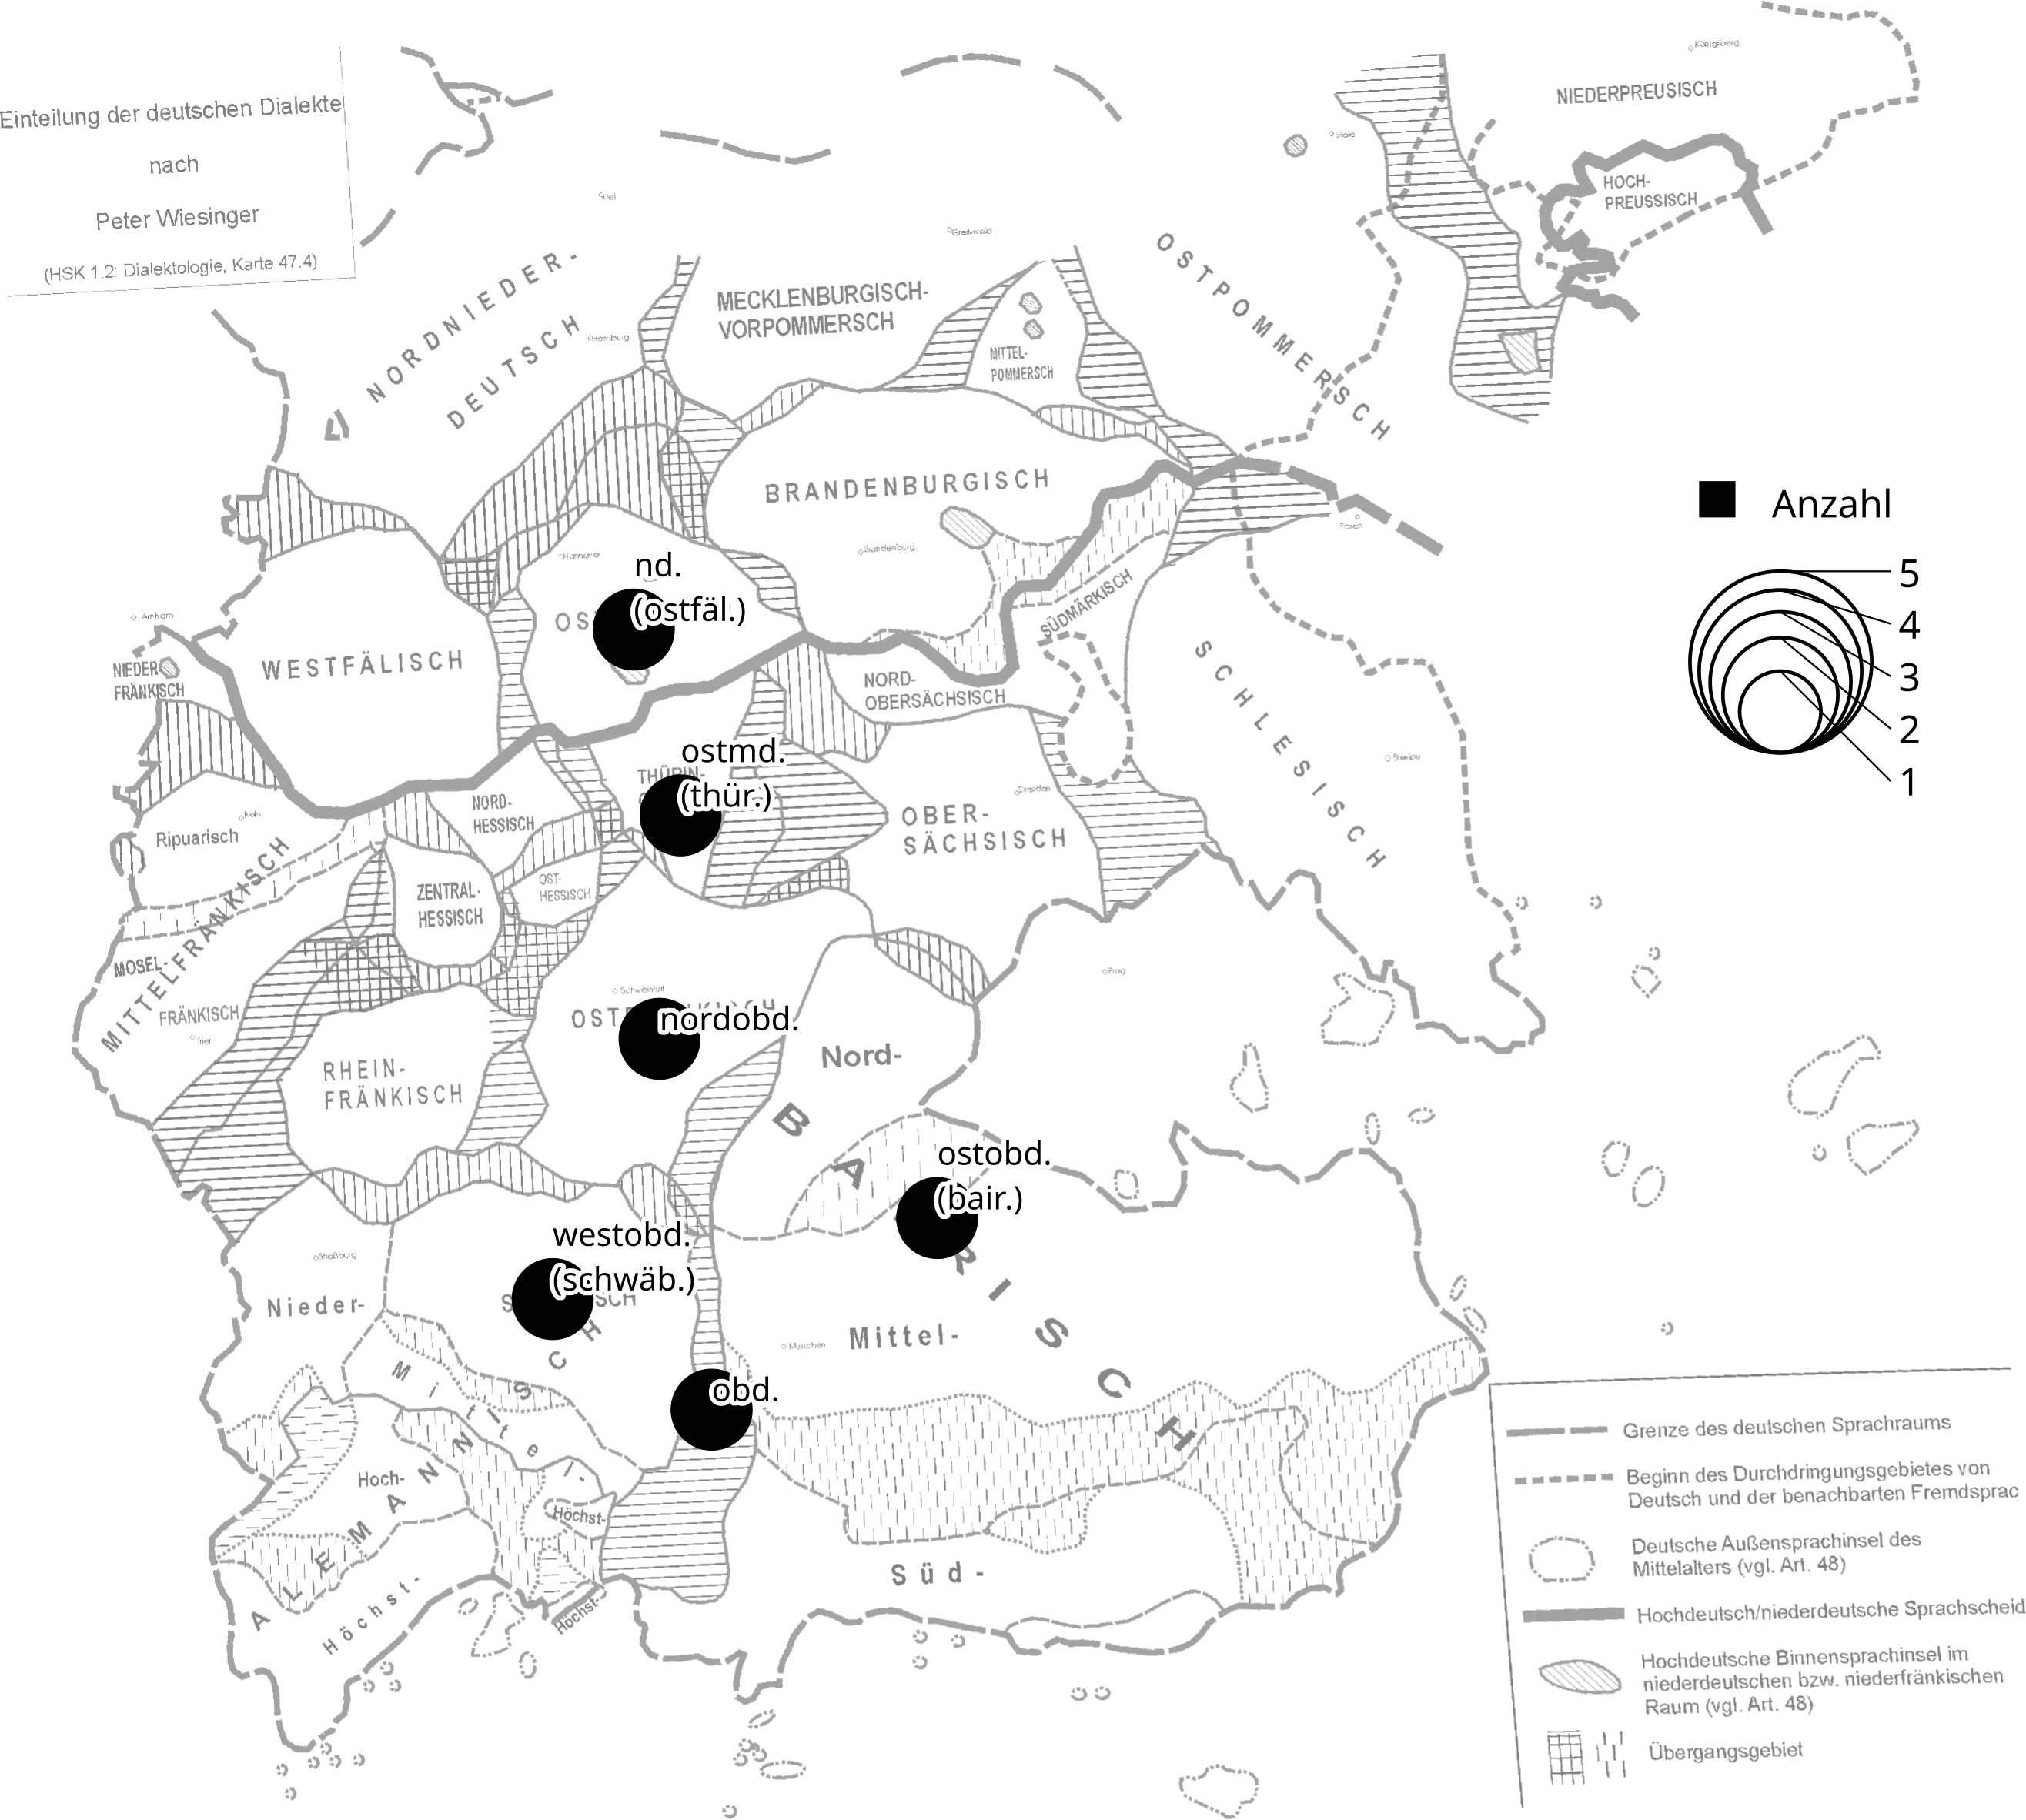
\includegraphics[
		width=.49\linewidth,
		height=.95\textheight,
		keepaspectratio
	]{./assets/grafiken/2021-12-30_kc_geospac_rough_c15.png}
}
\caption%
	[]
	{Grobe räumliche und zeitliche Verteilung der \citet{kc}-Textzeugen
		(Fortsetzung)\nocite{wiesinger1983:rede}
	}
	% \label{fig:kc_geospac_rough_2}
\end{figure}
\end{landscape}%
}

Die handschriftliche Überlieferung der \citet{kc} bietet also ein
entscheidendes Merkmal der geschäftsmäßigen Schriftlichkeit (Urkunden, Urbare)
oftmals gerade nicht: Autornähe. Des Weiteren sind die Handschriften der
\citet{kc} im Gegensatz zu den Urkunden des \citetitle{cao} weder exakt datiert
noch einigermaßen genau lokalisierbar. Aufgrund der von
\citet[1310]{wegera2000} angesprochenen \q*{Vorlagenproblematik} muss außerdem
tendenziell davon ausgegangen werden, dass Dialekt\-mischungen eher die Regel
als die Ausnahme darstellen. Der Vergleich der Daten aus der Auswertung der
\citet{kc} mit denen der \citetitle{cao}-Auswertung verspricht also besonders
valide Ergebnisse, insofern sich mit Hilfe der Urkunden regionale Merkmale von
Schreibdialekten verorten lassen, trotz der grundsätzlichen
Schreiberproblematik und der Einschränkung, dass die Urkunden lediglich eine
Momentaufnahme der geschriebenen Geschäftssprache des späten 13.~Jahrhunderts
darstellen.

Bezüglich der regionalen Variation von Schreibdialekten weist \citet{solms2014}
darauf hin, \blockcquote[132]{solms2014}{dass es die überaus große
Zersplitterung des Sprachgebietes, wie sie die Dialektgeographie des
19.~Jahrhunderts erwiesen hat, in der Schreibsprachlichkeit des 11.\ bis
14.~Jahrhunderts noch nicht gegeben hat}. Andererseits lässt sich fragen,
inwiefern die angesprochene Zersplitterung ein Artefakt der Erhebungsmethode
etwa von Sprachatlanten darstellt. Dialektgeografische Karten bilden nie die
Gesamtheit der Sprecherinnen und Sprecher mit sämtlichen Variations\-ebenen ab,
sondern unterliegen notwendigerweise Abstraktionen und Vereinfachungen, auch
durch die Auswahl der Informantinnen und Informanten. Diese
Komplexitätsreduktion produziert unter Umständen scharfe Grenzen, wo Übergänge
in der Realität fließend sind.
